\chapter{Work Methodology} \label{chapter_four}

So far we have discussed the problem we are trying to solve, what are the methods available to us and the challenges associated with them. This chapter contains the process we used to digitally stabilize video for our use-case. Figure \ref{fig:dis_pipeline} shows the pipeline we are using to digitally stabilize videos in our case.

% \begin{sidewaysfigure}
%     \centering
%     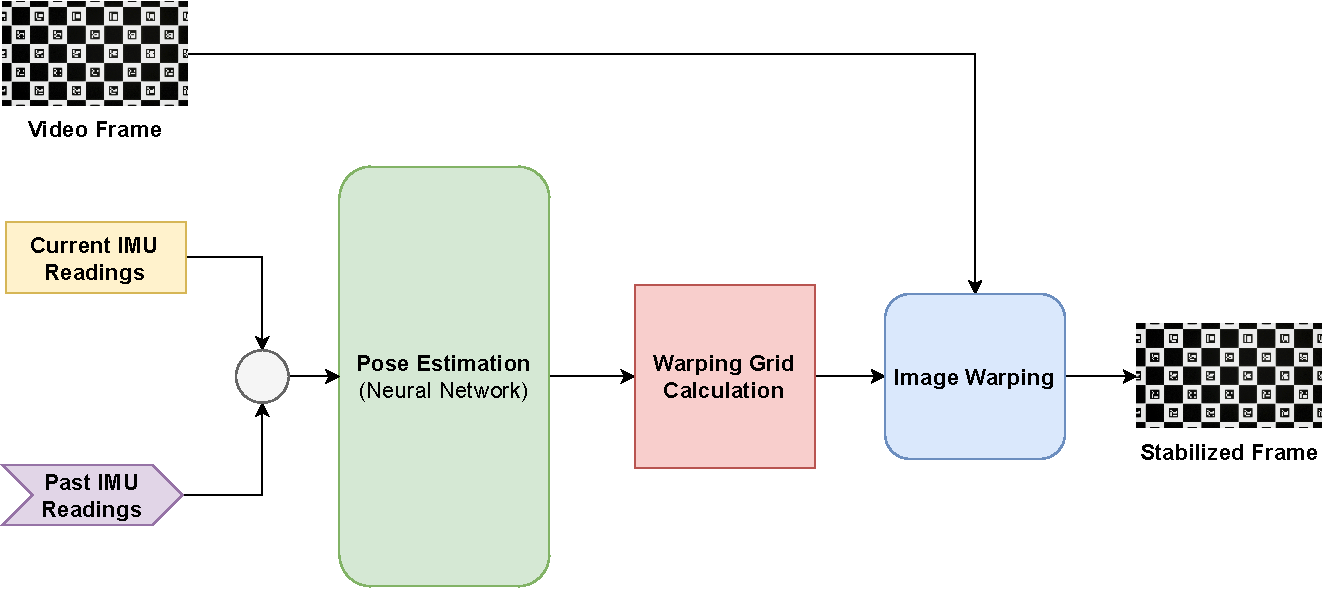
\includegraphics[scale=0.9]{images/fig_chapter4/dis_pipleline.pdf}
%     \caption{DIS pipeline using IMU Sensor}
%     \label{fig:dis_pipeline}
% \end{sidewaysfigure}

\begin{figure}[H]
    % \centering
    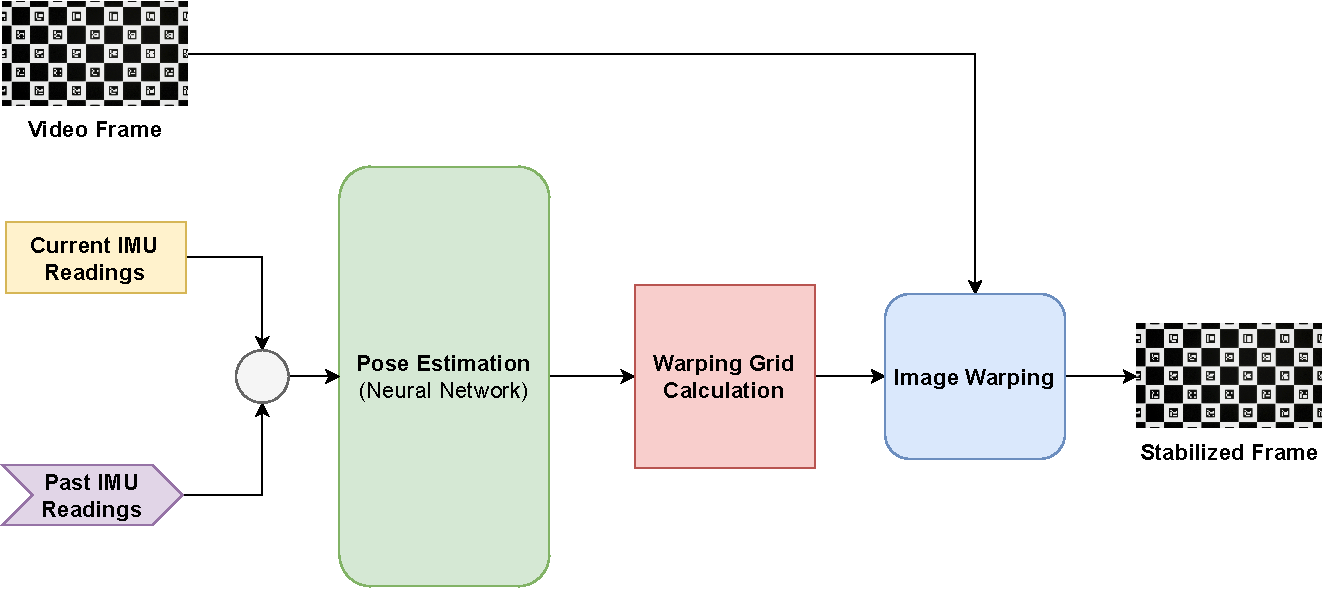
\includegraphics[scale=0.58]{images/fig_chapter4/dis_pipleline.pdf}
    \caption{DIS pipeline using IMU Sensor}
    \label{fig:dis_pipeline}
\end{figure}

We will be using an IMU sensor for camera pose estimation to stabilize the video for this work. Based on the precision requirements of the pose-estimation algorithm we will be using a data-driven approach as classical signal processing and sensor fusion algorithms fail to provide this precision over a long period of time. For our data driven approach we build datasets using a camera and also simulation. To capture the video we are using a GoPro Hero 10 which provides synchronised image and sensor data capture. We also swapped the factory lens to a low Field of View (FOV) and high focal length lens (figure \ref{fig:mod_gopro_hero10}). The simulation was build using Unreal Engine 4 and Microsoft AirSim. Table \ref{tab:technical_details} shows the technical specifications of the camera setup. For simulation similar camera parameters were used.

\begin{table}[H]
    \centering
\begin{tabular}{ c| c | L }

     Image Sensor & 
     Sony & 
     Diagonal 7.85 mm (Type 1/2.3) 23.91 M CMOS Image Sensor with Square Pixel. \\
     \hline
     
     IMU Sensor & 
     Bosch & 
     6-axis IMU Sensor
     Accelerometer (A): 16-bit or 0.06 mg/LSB 
     Gyroscope (G): 16-bit or 0.004 dps/LSB  \\
     \hline
     
     Lens & 
     xx & 
     15° FOV and 200 mm focal length \\

\end{tabular}
    \caption{Hardware technical specifications}
    \label{tab:technical_details}
\end{table}

\begin{figure}[H]
    \centering
    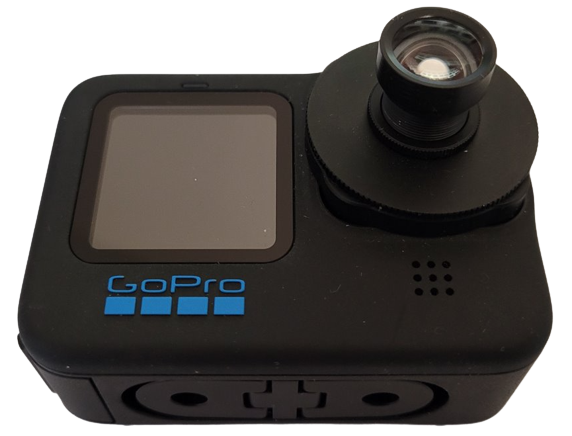
\includegraphics[scale=0.25]{images/fig_chapter4/mod_gorpro_hero_10.png}
    \caption{Modified GoPro Hero 10 with Low FOV and High Focal length lens}
    \label{fig:mod_gopro_hero10}
\end{figure}

\begin{figure}[H]
    \centering
    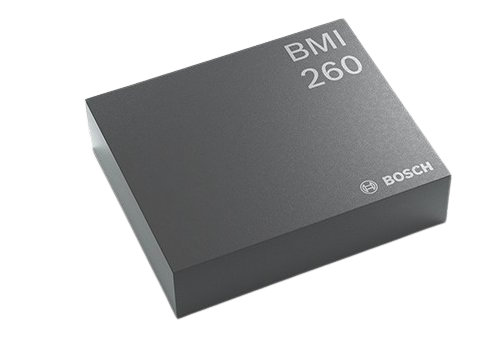
\includegraphics[scale=0.2]{images/fig_chapter4/bmi260.png}
    \caption{Bosch BMI260 IMU Sensor}
    \label{fig:imu_bmi260}
\end{figure}

\section{Data Collection}
Collecting data for any data driven approach is a challenging and an iterative process. The data or training data in this case are the readings coming from the IMU sensor and the target (ground truth) being the camera pose (position and orientation). Real data was collected by mounting the camera on a rig which had vibrations associated with it on movement (figure \ref{fig:camera_rig}). We made sure that the data depicts real life scenarios by moving the rig around in many different ways and let it vibrate and collect the data. The ground truth was generated using proprietary Zeiss software and is beyond the scope of this work. 

\begin{figure}[H]
    \centering
    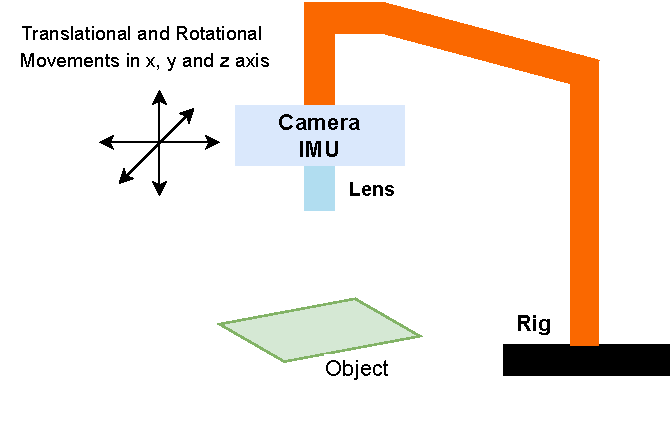
\includegraphics[scale=0.8]{images/fig_chapter4/camera_rig.pdf}
    \caption{Camera rig setup}
    \label{fig:camera_rig}
\end{figure}

Then the data was collected from simulation based on the analysed real data and pushed beyond real data limits to account for even more challenging scenarios. Generating simulated data with accurate ground truth is a fast processes not requiring much post-processing. This also allowed us to tinker with noise and bias to make the neural network robust and generalize well.

\subsection{Data Analysis}
\label{data_analysis}
The data recorded from a camera-rig setup was analysed to determine the vibration and sensor parameters. Table \ref{tab:imu_noise_characteristics} summarises the white noise and bias characteristics determined from the raw IMU Sensor Readings. These match closely with the data provided by the manufacturer. Accelerometer variance from data sheet $ 160 \mu g /\sqrt{Hz} $ and for gyroscope $ 0.008 dps /\sqrt{Hz}  $.

\begin{table}[H]
\centering
\begin{tabular}{l|c}
    \textbf{Parameter} & \textbf{Value} \\ \hline
    Accelerometer Bias & xx \\  
    Accelerometer White Noise & $ \mu = 0 $ and $ \sigma^{2}=0.00038 m/s^{2}$ \\  
    Gyro Bias & xx \\  
    Gyro White Noise & $ \mu = 0 $ and $ \sigma^{2}=0.xxx $ \\  
\end{tabular}
\caption{IMU Noise Characteristics}
\label{tab:imu_noise_characteristics}
\end{table}

We analysed the generated ground truth to determine the characteristics of vibration. These characteristics are important to understand the nature of vibration and to set the working limits for our work. Vibrations are characterised by \textbf{Amplitude} ( A or  $ \theta $), \textbf{Time Constant} ($ \tau $) and \textbf{Frequency} ($ \omega $). We have damped oscillations for both displacement and rotation vibration as shown in figure \ref{fig:damped_vib} and can be characterised by the equations \ref{eqn:vib_disp} and \ref{eqn:vib_rot}.

\begin{equation}
  \label{eqn:vib_disp}
  \begin{aligned}
    A(t) = Ae^{-t/\tau}sin(2\pi\omega t) \\
  \end{aligned}
\end{equation}

\begin{equation}
  \label{eqn:vib_rot}
  \begin{aligned}
    \theta(t) = \theta e^{-t/\tau}sin(2\pi\omega t) \\
  \end{aligned}
\end{equation}

\begin{figure}[H]
    \centering
    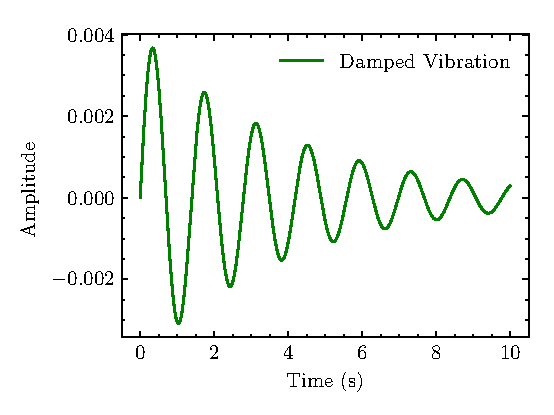
\includegraphics{images/fig_chapter4/vib_damped.eps}
    \caption{Damped Vibration}
    \label{fig:damped_vib}
\end{figure}

%% Displacement distribution
\begin{figure}[H]
    %%
    \begin{subfigure}{\linewidth}
    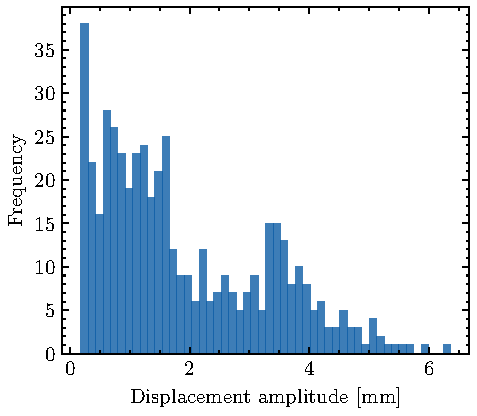
\includegraphics[width=.5\linewidth]{images/fig_chapter4/data_dist/1.pdf}\hfill
    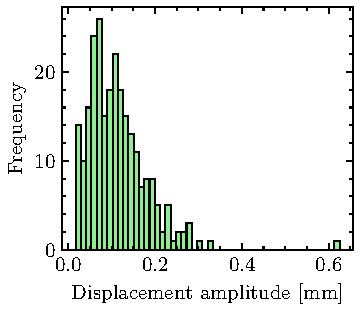
\includegraphics[width=.5\linewidth]{images/fig_chapter4/data_dist/2.pdf}
    \caption{Distribution of displacement amplitude $ A $ in XY(left) and Z(right) DoF [mm]}
    \end{subfigure}\par\medskip
    
    %%
    \begin{subfigure}{\linewidth}
    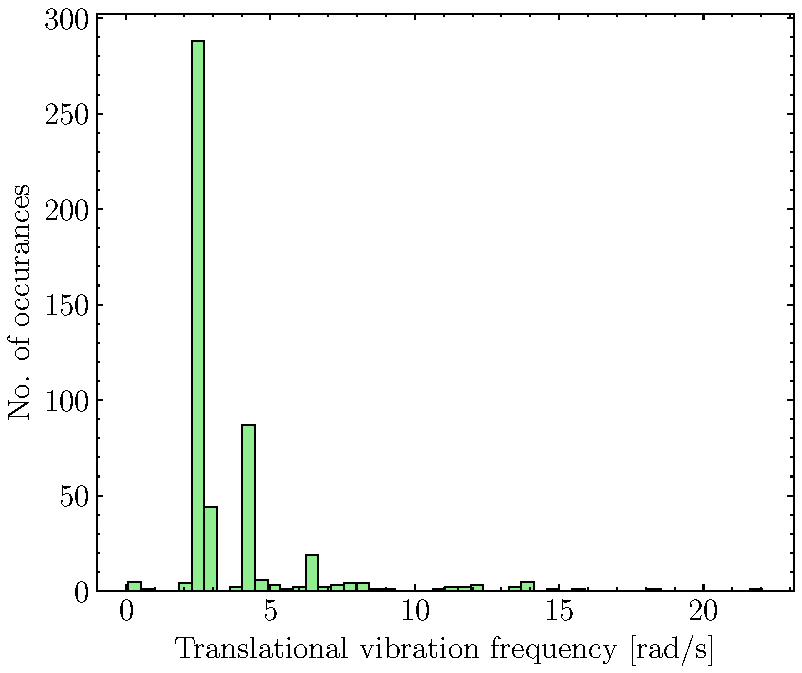
\includegraphics[width=.5\linewidth]{images/fig_chapter4/data_dist/3.pdf}\hfill
    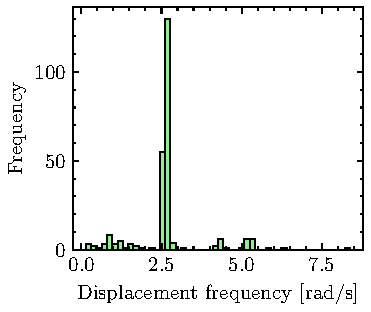
\includegraphics[width=.5\linewidth]{images/fig_chapter4/data_dist/4.pdf}
    \caption{Distribution of displacement frequency $ \omega $ in XY(left) and Z(right) DoF [mm]}
    \end{subfigure}\par\medskip
    
    %%
    \begin{subfigure}{\linewidth}
    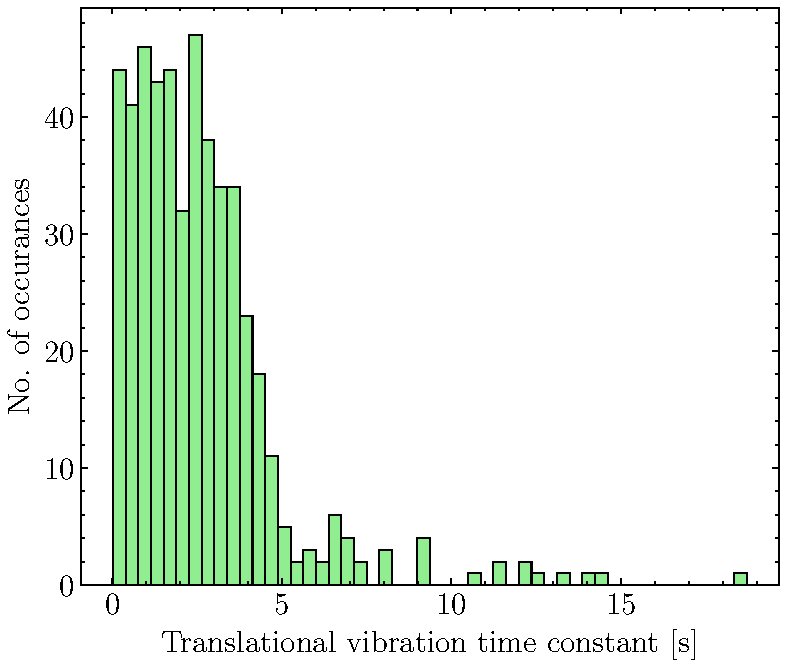
\includegraphics[width=.5\linewidth]{images/fig_chapter4/data_dist/5.pdf}\hfill
    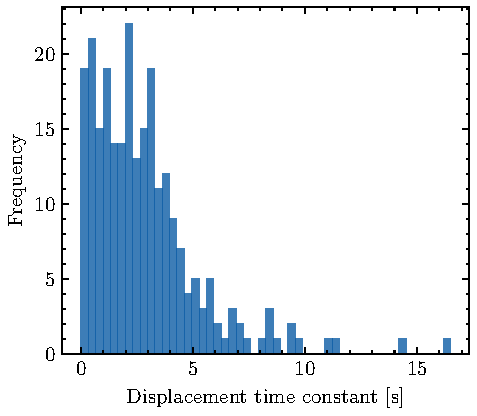
\includegraphics[width=.5\linewidth]{images/fig_chapter4/data_dist/6.pdf}
    \caption{Distribution of displacement time-constant $ \tau $ in XY(left) and Z(right) DoF [mm]}
    \end{subfigure}
\caption{Real displacement data statistical analysis}
\label{fig:dist_disp}
\end{figure}

%% Rotation Distribution 
\begin{figure}[H]
    %%
    \begin{subfigure}{\linewidth}
    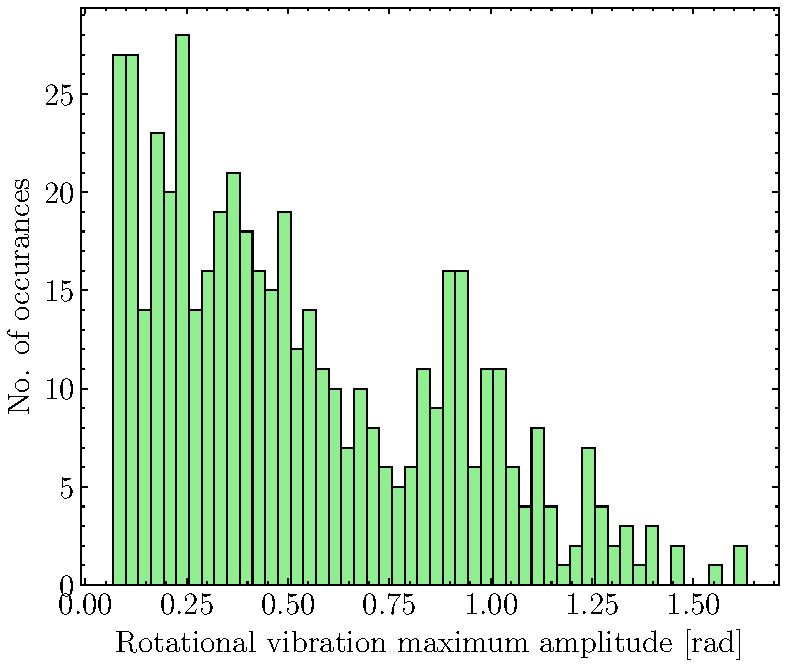
\includegraphics[width=.5\linewidth]{images/fig_chapter4/data_dist/7.pdf}\hfill
    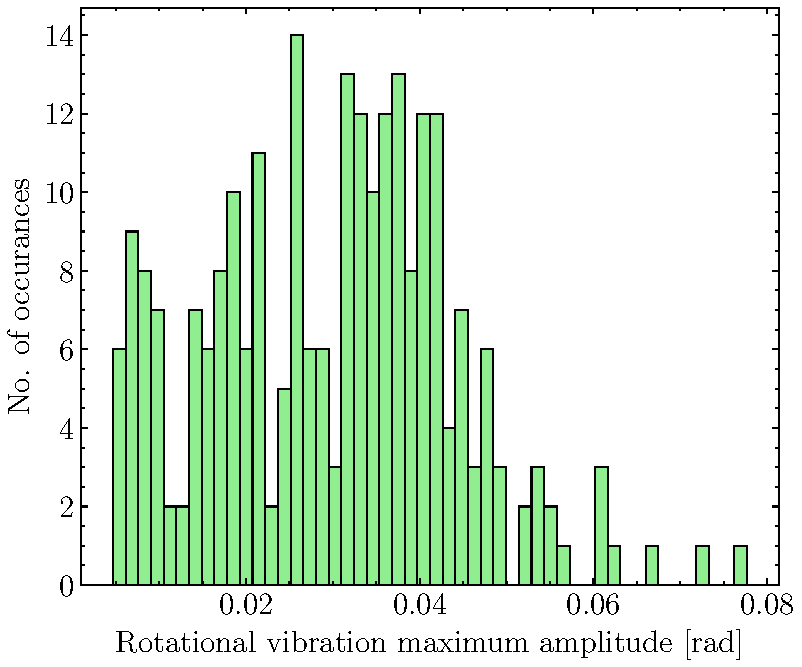
\includegraphics[width=.5\linewidth]{images/fig_chapter4/data_dist/8.pdf}
    \caption{Distribution of rotation amplitude $ \theta $ in XY(left) and Z(right) DoF [mm]}
    \end{subfigure}\par\medskip
    
    %%
    \begin{subfigure}{\linewidth}
    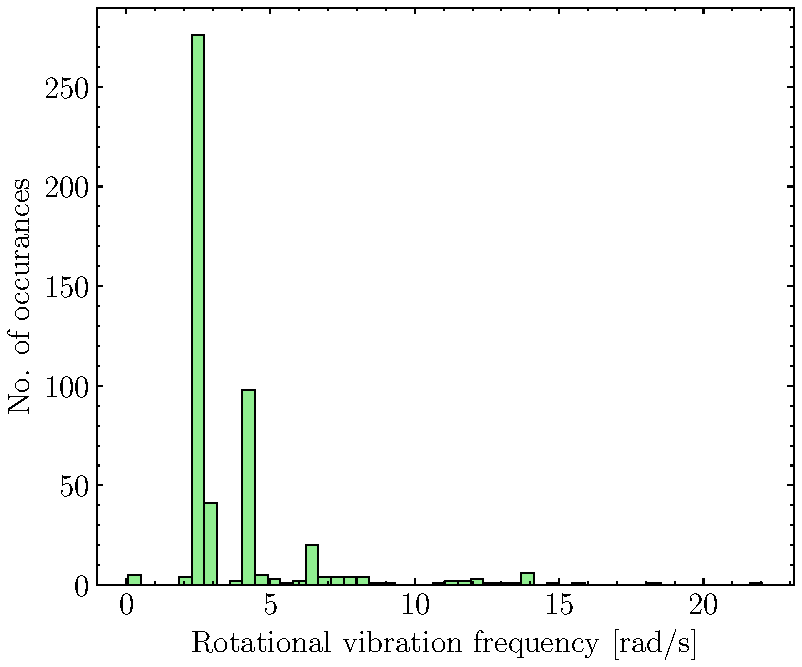
\includegraphics[width=.5\linewidth]{images/fig_chapter4/data_dist/9.pdf}\hfill
    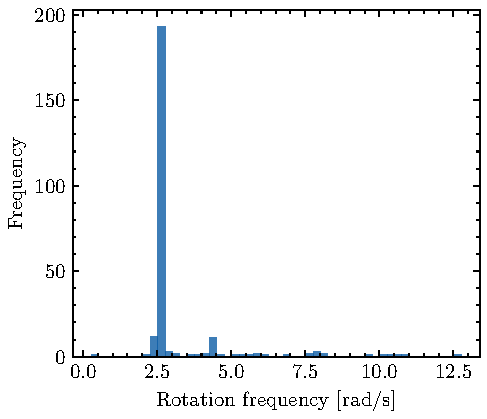
\includegraphics[width=.5\linewidth]{images/fig_chapter4/data_dist/10.pdf}
    \caption{Distribution of rotation frequency $ \omega $ in XY(left) and Z(right) DoF [mm]}
    \end{subfigure}\par\medskip
    
    %%
    \begin{subfigure}{\linewidth}
    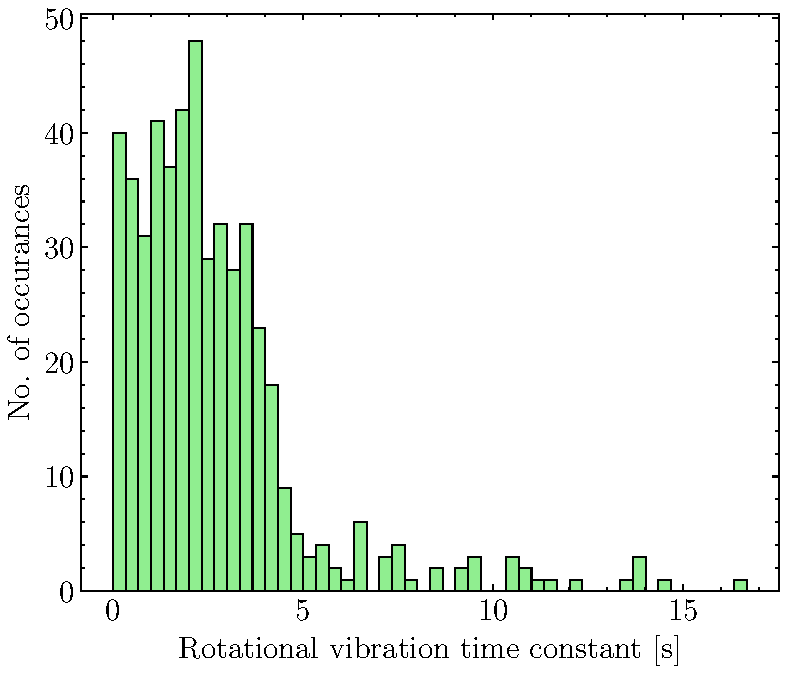
\includegraphics[width=.5\linewidth]{images/fig_chapter4/data_dist/11.pdf}\hfill
    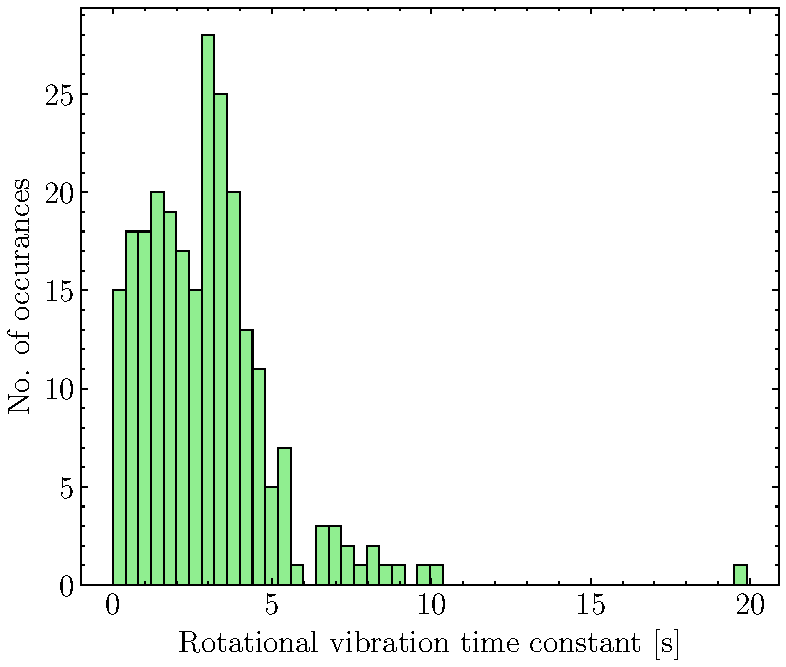
\includegraphics[width=.5\linewidth]{images/fig_chapter4/data_dist/12.pdf}
    \caption{Distribution of rotation time-constant $ \tau $ in XY(left) and Z(right) DoF [mm]}
    \end{subfigure}

\caption{Real rotation data statistical analysis}
\label{fig:dist_rot}
\end{figure}


The statistical analysis shown in figure \ref{fig:dist_disp} and figure \ref{fig:dist_rot} was done on 248 vibration sequences with an average length of 10 seconds. The results for displacement and rotation vibrations are summarised in table \ref{tab:real_data_analysis_displacement} and table \ref{tab:real_data_analysis_rotation} respectively. The rotational vibrations have very small amplitude ($ \theta $) and is less than 1 degrees for more than 75 percent of the samples in XY plane. For Z axis the vibrations are even smaller with a mean of 0.0005 degrees. These vibrations are very small and do not have a a noticeable visual effect on the video stabilization. But we have decided to account for them to develop a more general solution with multiple applications. The time constant ($ \tau $) for displacement and rotation is similar for all DoF with a mean value of around 2.9 seconds.  The frequency ($ \omega $) for all DoF is also similar in the range $ 2.5 rad/sec $ to $ 3.5 rad/sec $. Frequency of $ 2.5 rad/sec $ is the most dominant frequency and seems to be the natural frequency $ \omega_n $ of the mechanical system (rig on which the camera is mounted).


The amplitude ($ A $) of the vibration displacement is the most important characteristic for this work as it is main source of video destabilization. The effect of motion on the quality of video is more pronounced in XY plane as the most pixel shift happens here. In Z axis the mean ($ \mu $) of vibrations is 0.113 mm with a standard deviation ($ \sigma^{2} $) of 0.07 mm. Even the large vibrations in Z seem to have little effect on visual quality of the video. Vibrations in XY plane have the mean of 1.9 mm with a standard deviation of 1.36 mm. Vibrations with higher magnitude are also present and need to be accounted for when generating simulated data.

% displacement data distribution table
\begin{table}[H]
    \centering
\begin{tabular}{ c | L | L | L }
    
     Parameter  & 
     Mean ($ \mu $) & 
     Variance ($ \sigma^{2} $) &
     Standard Deviation ($ \sigma $)\\
     \hline
     
     $ A_{xy} $ & 
     $ 1.8944 mm $ & 
     $ 1.8674 mm^{2} $ &
     $ 1.3665 mm $ \\

      
     $ A_{z} $  & 
     $ 0.1135 mm $ & 
     $ 0.0047 mm^{2} $ &
     $ 0.0690 mm $ \\
     
     
     $ \omega_{xy} $ & 
     $ 3.6898 rad/s $ & 
     $ 5.9833 rad^{2}/s^{2} $ &
     $ 2.4460 rad/s $ \\
     
     
     $ \omega_{z} $& 
     $ 2.6835 rad/s $ & 
     $ 2.0765 rad^{2}/s^{2} $ &
     $ 1.0375 rad/s $ \\

     
     $ \tau_{xy} $ & 
     $ 2.5914 s $ & 
     $ 5.1898 s^{2} $ &
     $ 2.2781 s $ \\


     $ \tau_{z} $ & 
     $ 2.8396 s $ & 
     $ 5.8720 s^{2} $ &
     $ 2.4243 s $ \\

\end{tabular}
    \caption{Real Data displacement-vibration distributions}
    \label{tab:real_data_analysis_displacement}
\end{table}

% rotation data distribution table
\begin{table}[H]
    \centering
\begin{tabular}{ c | L | L | L }

     Parameter  & 
     Mean ($ \mu $) & 
     Variance ($ \sigma^{2} $) &
     Standard Deviation ($ \sigma $)\\
     \hline
     
     $ \theta_{xy} $ & 
     $ 0.0094 rad $ & 
     $ 3.8729e^{-8} rad^{2} $ &
     $ 0.0062 rad $ \\

      
     $ \theta_{z} $  & 
     $ 0.0005 rad $ & 
     $ 6.0739e^{-8} rad^{2} $ &
     $ 0.0002 rad $ \\
     
     
     $ \omega_{xy} $ & 
     $ 3.8042 rad/s $ & 
     $ 6.3685 rad^{2}/s^{2} $ &
     $ 2.5236 rad/s $ \\

     
     $ \omega_{z} $& 
     $ 3.1763 rad/s $ & 
     $ 2.6238 rad^{2}/s^{2} $ &
     $ 1.6198 rad/s $ \\
   
     
     $ \tau_{xy} $ & 
     $ 2.6581 s $ & 
     $ 5.8362 s^{2} $ &
     $ 2.4158 s $ \\
    
     
     $ \tau_{z} $ & 
     $ 2.9316 s $ & 
     $ 4.7336 s^{2} $ &
     $ 2.1757 s $ \\

\end{tabular}
    \caption{Real Data rotational-vibration distributions}
    \label{tab:real_data_analysis_rotation}
\end{table}



\subsection{Simulated Data Generation}
\label{sec:gen_sim_data}
The simulated data plays a very important role in our approach as we use the ideal data to validate our stabilization approach. It also empowers us to simulate IMU sensors with different noise levels and characteristics. We also made sure that the data generated from the simulation is fairly domain randomized to make it realistic. 

Simulated data is based on the analysed real data with vibration characteristics taken from table \ref{tab:real_data_analysis_displacement} and table \ref{tab:real_data_analysis_rotation}. The data is then generated using the equations \ref{eqn:vib_disp} and \ref{eqn:vib_rot} .The simulated data is then augmented with modified noise and bias characteristics from table \ref{tab:imu_noise_characteristics}. A total of 600 vibration sequences with an average vibration duration of 15 seconds was generated with characteristics shown in tables \ref{tab:real_data_analysis_displacement} and \ref{tab:real_data_analysis_rotation}. Generating a large number of samples ensures the sampling of diverse data from the distribution. This is where we benefit from our simulation the most as the diversity and the size of data ensures our neural network generalizes well.


\section{Structuring of Data}
\label{sec:data_structure}
In classical pose-estimation techniques, every single IMU sample is used individually along with initial condition. Data driven approaches differ in this case as discussed in section \ref{sec:sota_pose_est}. For data driven approaches instead of taking an individual sample a \textit{window} of samples (figure \ref{fig:imu_window_samples})is used as a single sample does not contain enough information. Neural Networks unlike classical mathematics based approaches are data hungry and look for patterns in data and based on these patterns they generate an output. Initially we experimented with small window samples (3 - 20 samples) as shown in figure \ref{fig:imu_window_samples} a. This did not yield very good results and the pose estimation error was higher than the required. It started giving good results once we reach a IMU \textbf{ window size} of 70 to 140 samples (figure \ref{fig:imu_window_samples}). Beyond these the performance does not improve much and the inferences from the neural network become computationally expensive and inference latency become very high.

\begin{figure}[H]
    %%
    \begin{subfigure}{\linewidth}
    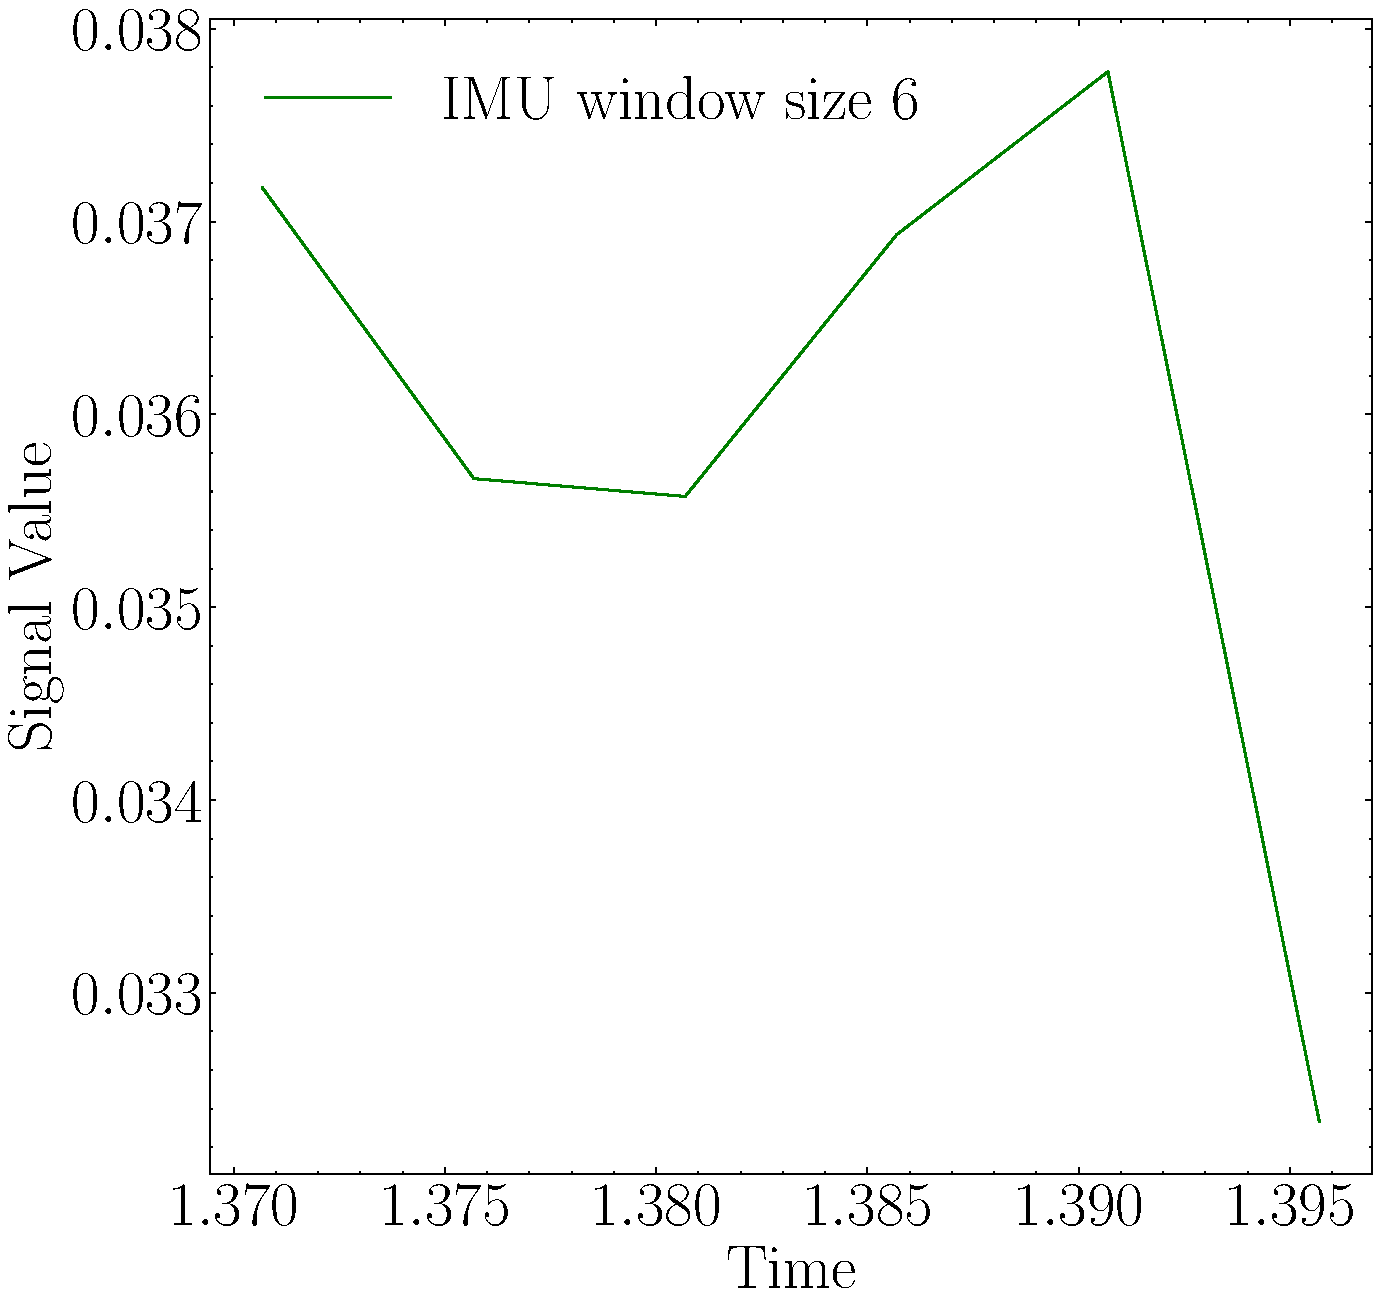
\includegraphics[width=.3\linewidth]{images/fig_chapter4/imu_windows/imu_window_size_6.pdf}\hfill
    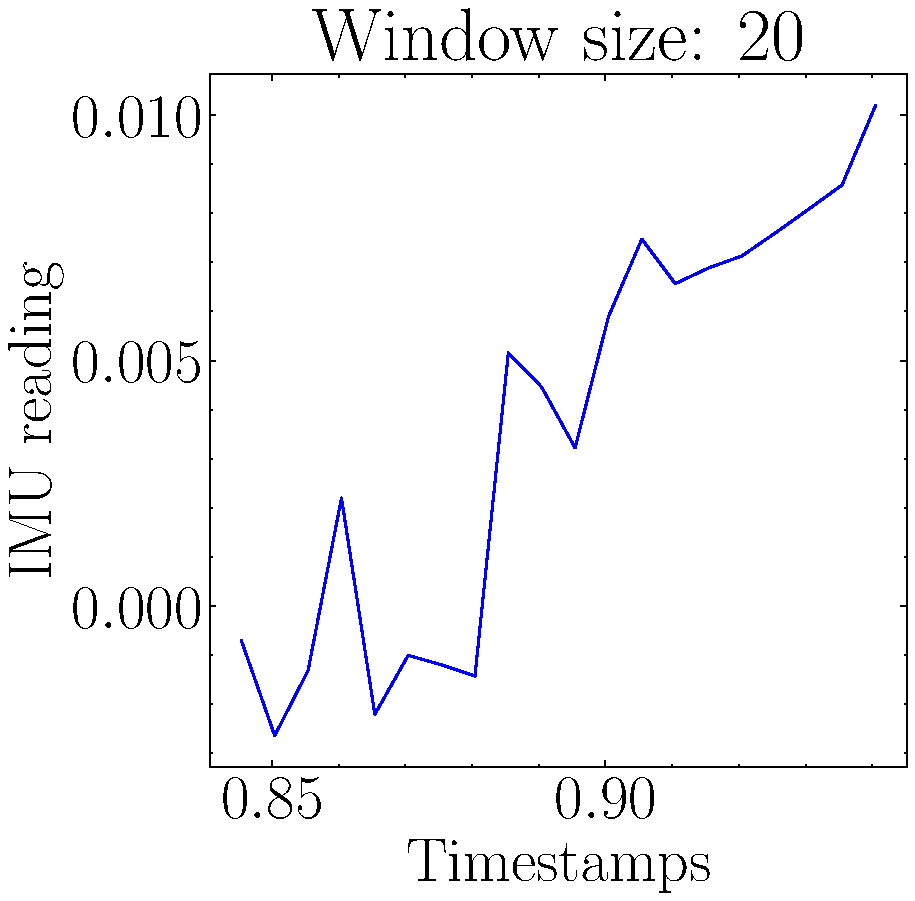
\includegraphics[width=.3\linewidth]{images/fig_chapter4/imu_windows/imu_window_size_20.pdf}\hfill
    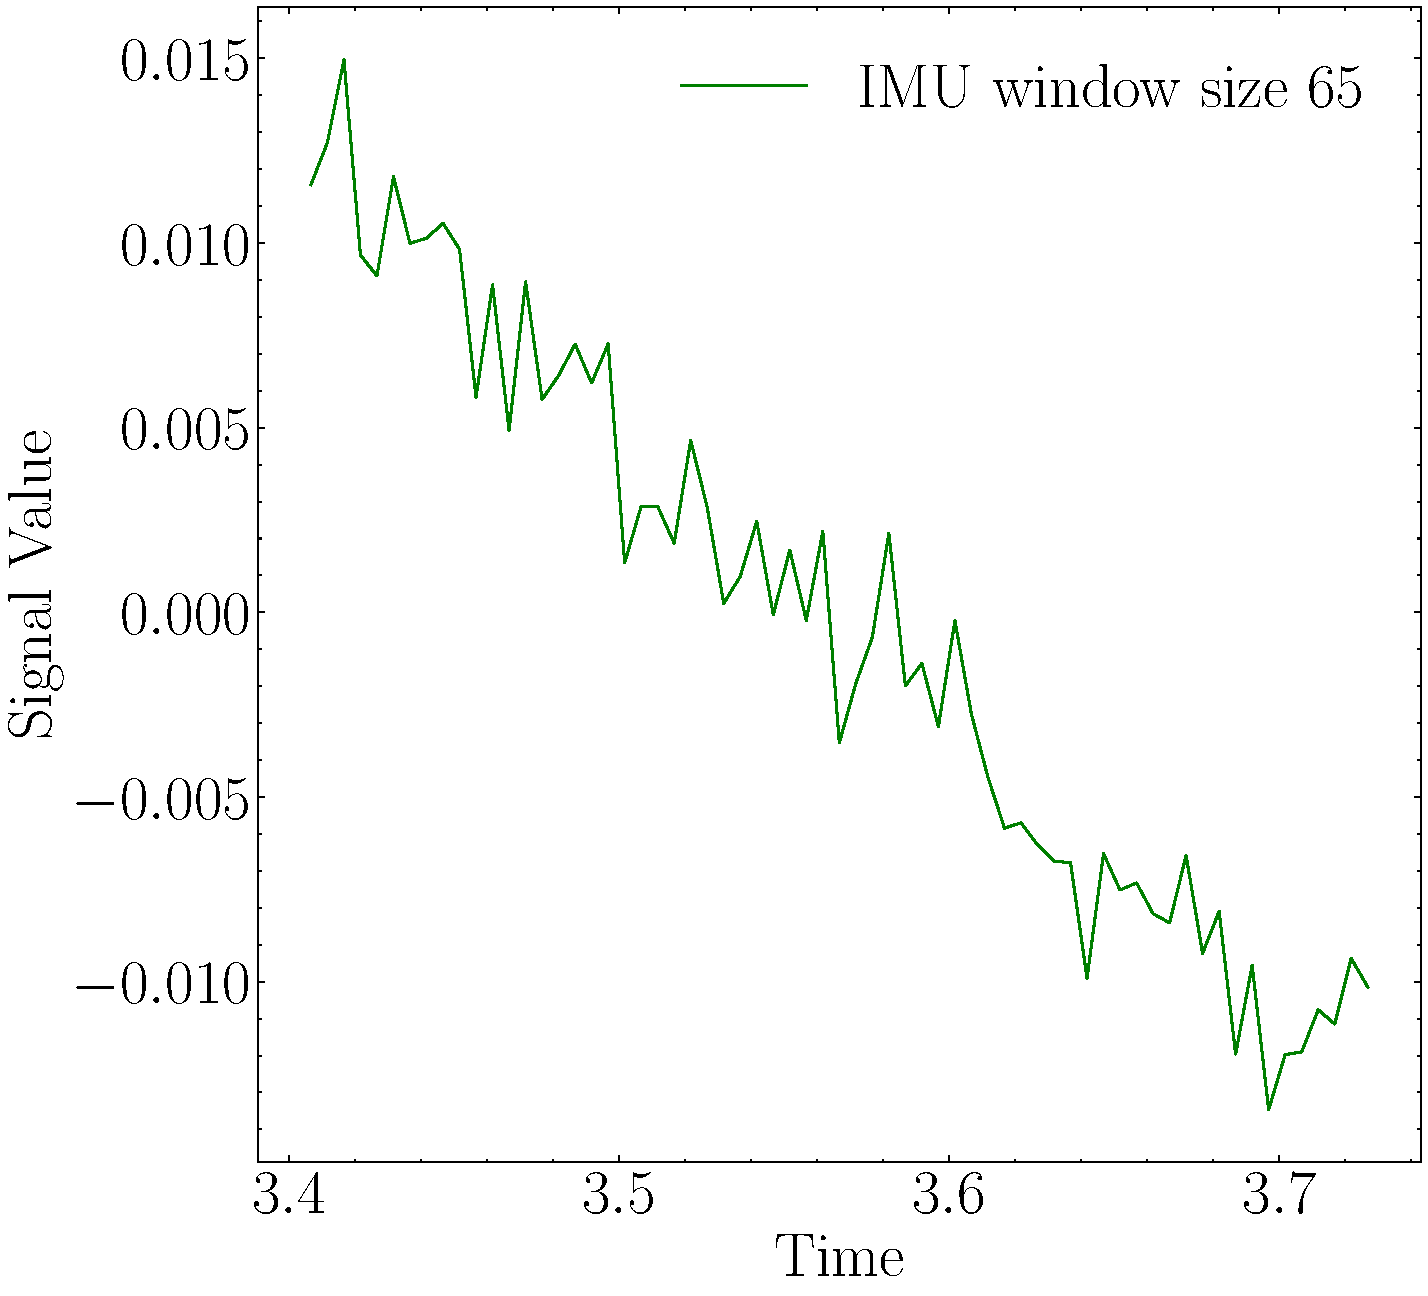
\includegraphics[width=.3\linewidth]{images/fig_chapter4/imu_windows/imu_window_size_65.pdf}\hfill
    \caption{Window size 6, 20 and 65}
    \end{subfigure}\par\medskip
    
    %%
    \begin{subfigure}{\linewidth}
    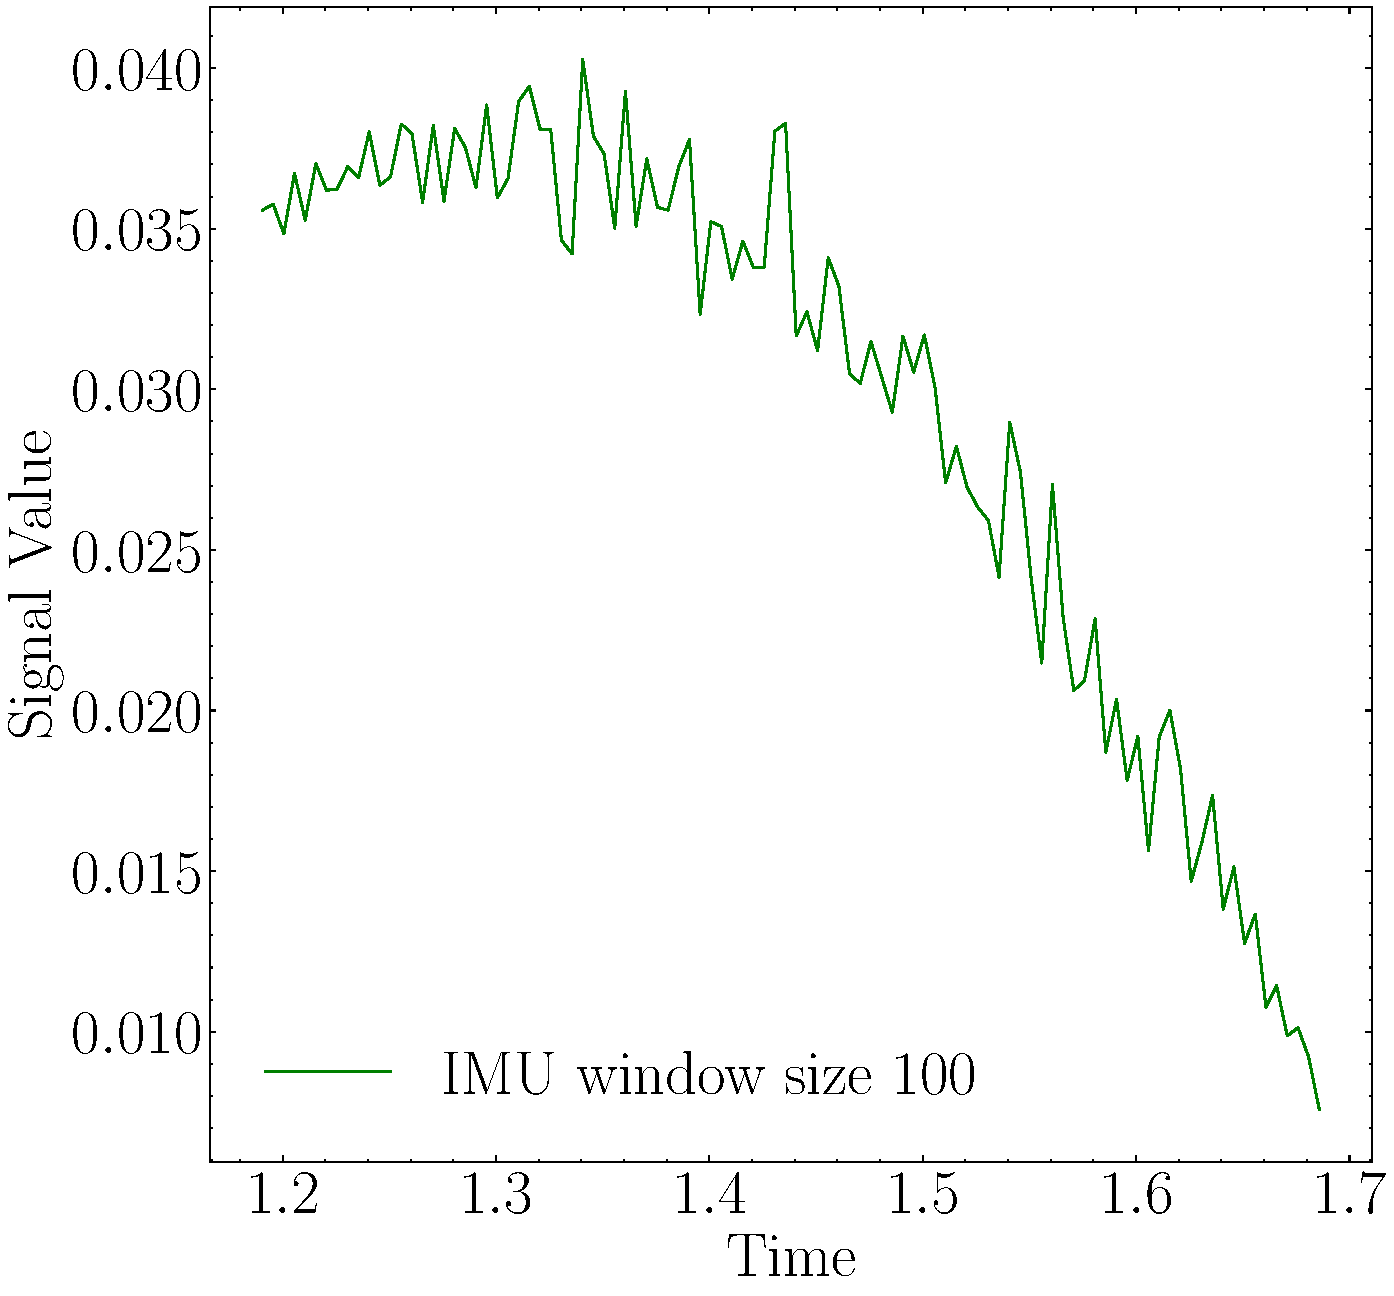
\includegraphics[width=.3\linewidth]{images/fig_chapter4/imu_windows/imu_window_size_100.pdf}\hfill
    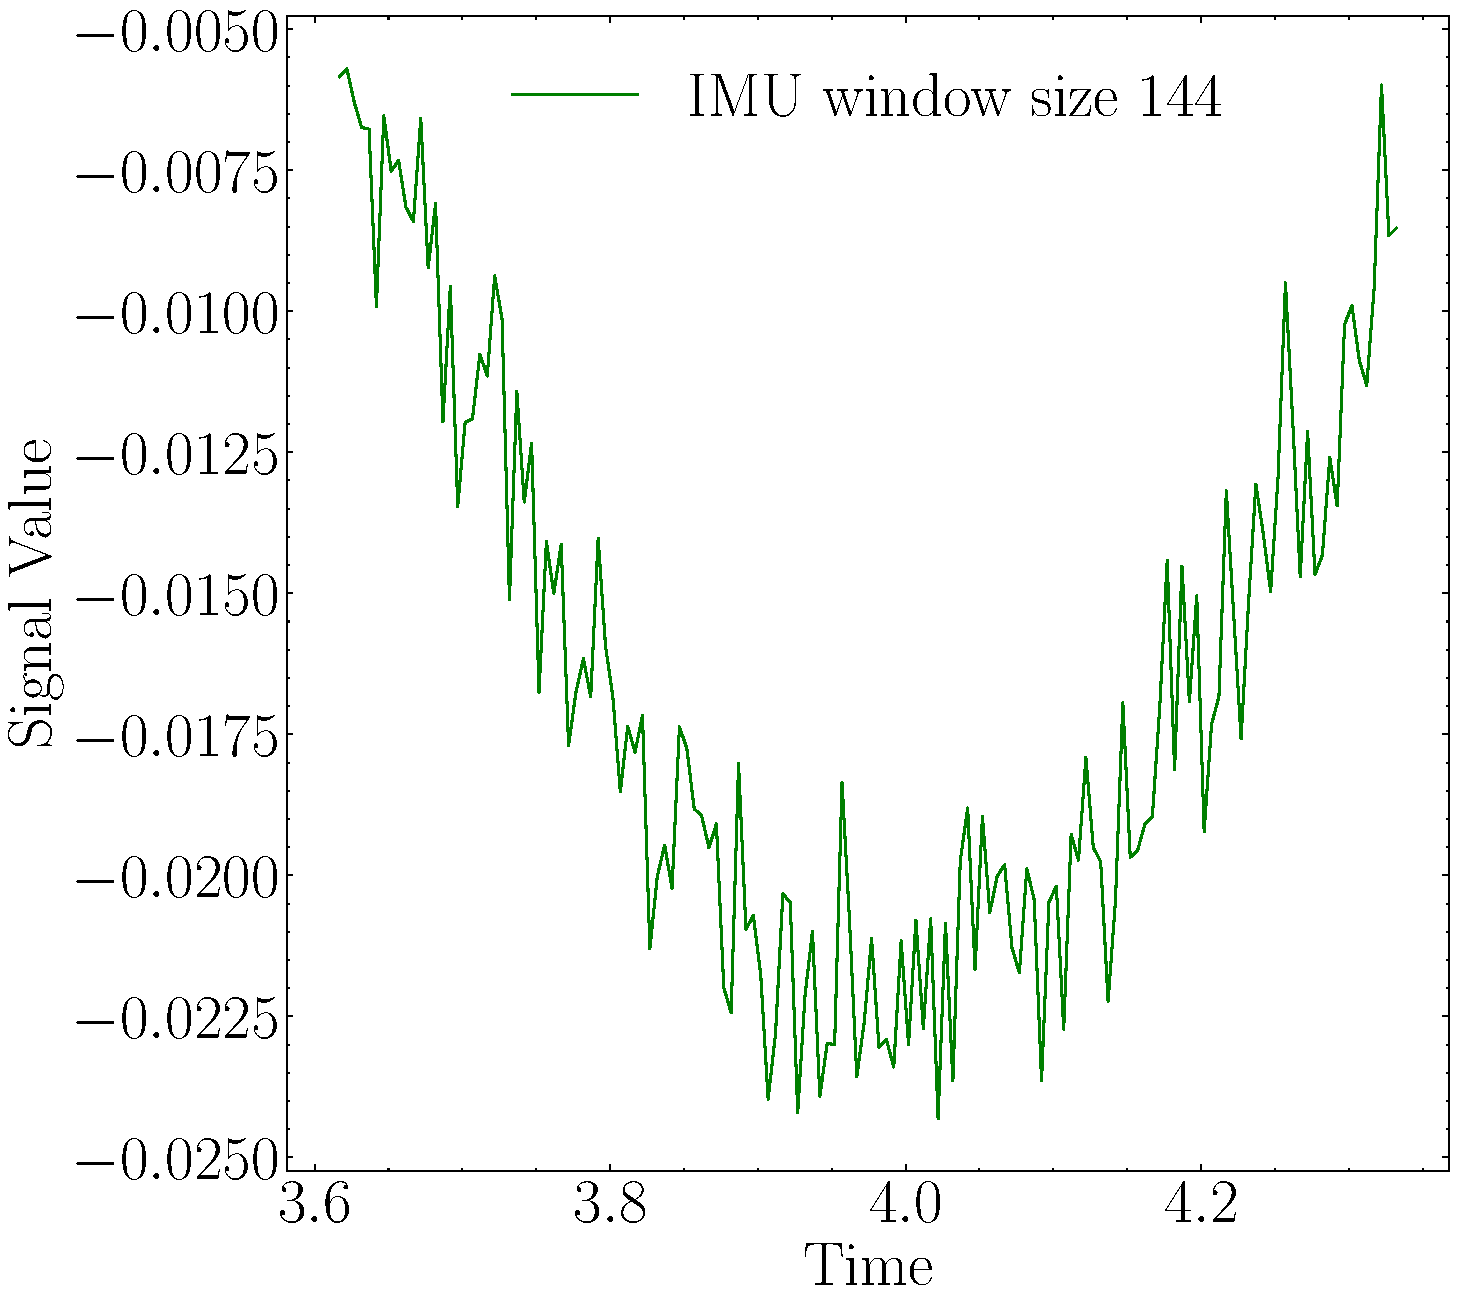
\includegraphics[width=.3\linewidth]{images/fig_chapter4/imu_windows/imu_window_size_144.pdf}\hfill
    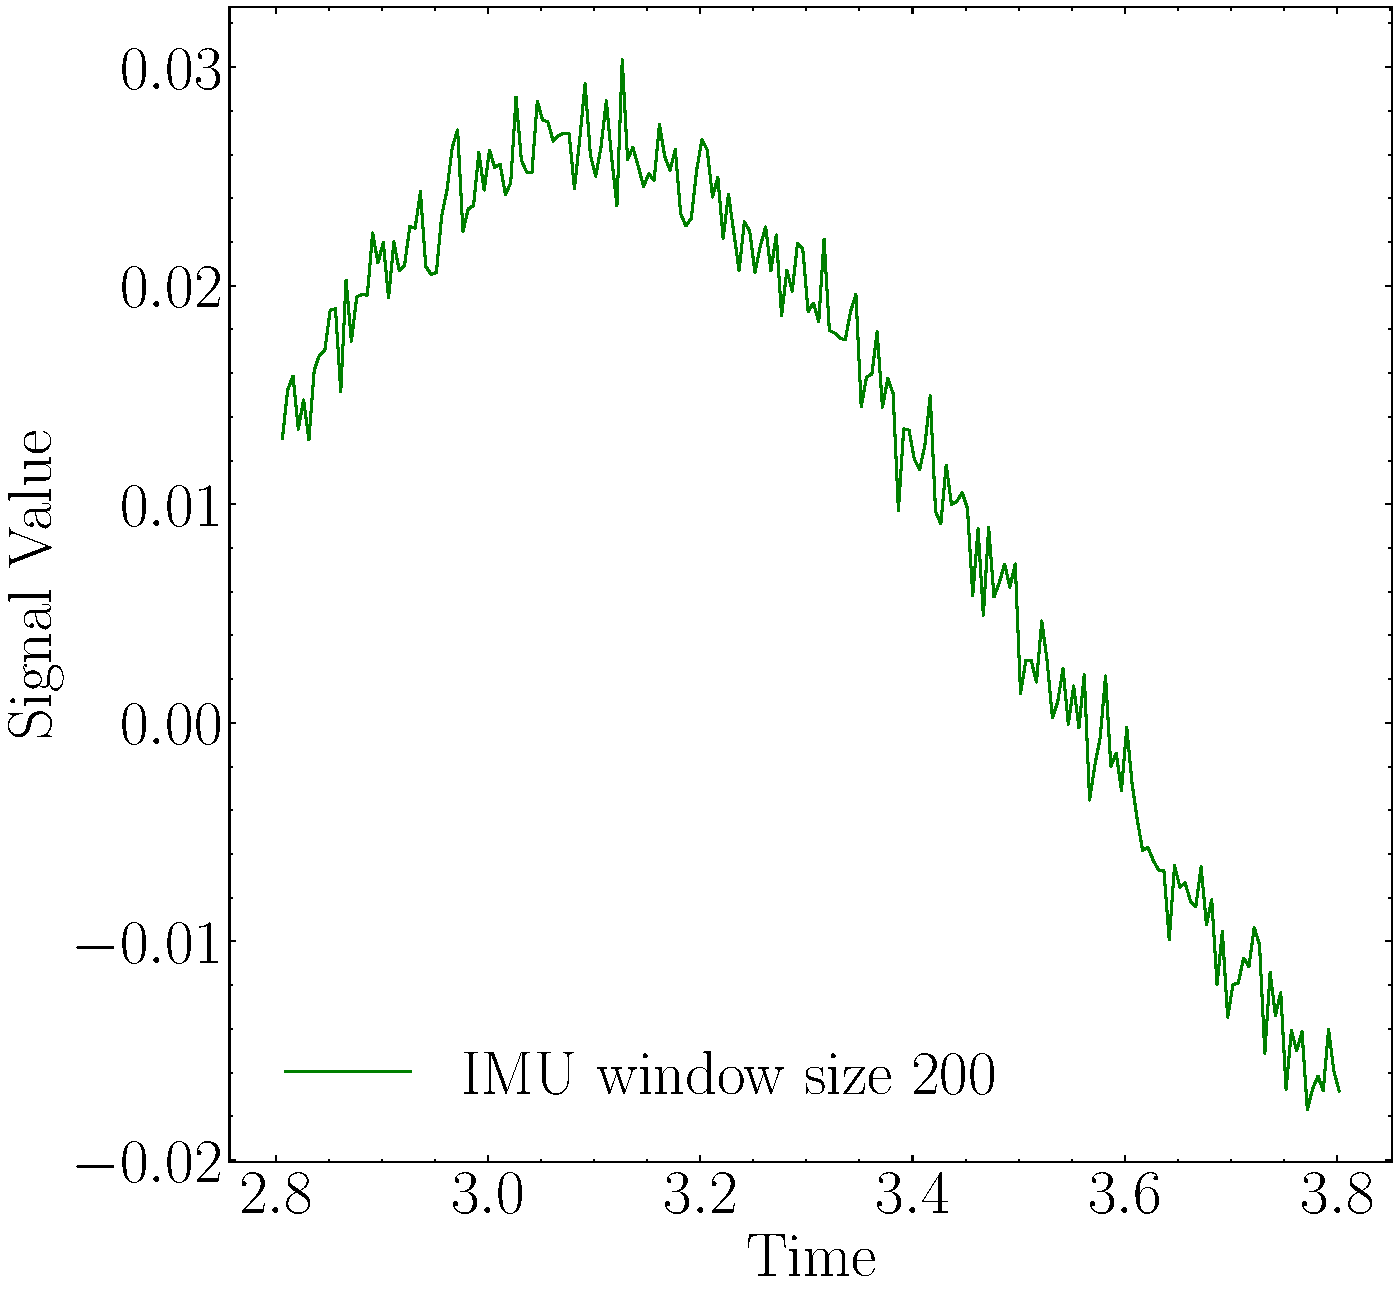
\includegraphics[width=.3\linewidth]{images/fig_chapter4/imu_windows/imu_window_size_200.pdf}\hfill
    \caption{Window size 100, 144, 200}
    \end{subfigure}
\caption{Different IMU window samples}
\label{fig:imu_window_samples}
\end{figure}

\section{Training and Testing of Various Neural Networks}
Various neural networks architectures were trained and tested to accurately estimate the camera pose with respect to a stabilised trajectory. Network takes as input the sensor readings coming from an IMU and the network is trained against the deviation with respect to stabilization trajectory. The stabilization trajectory can be realised as a mean of the vibration displacement (linear/angular) for an ideal case as shown in figure \ref{fig:stab_traj_ideal}. 

\begin{figure}
    \centering
    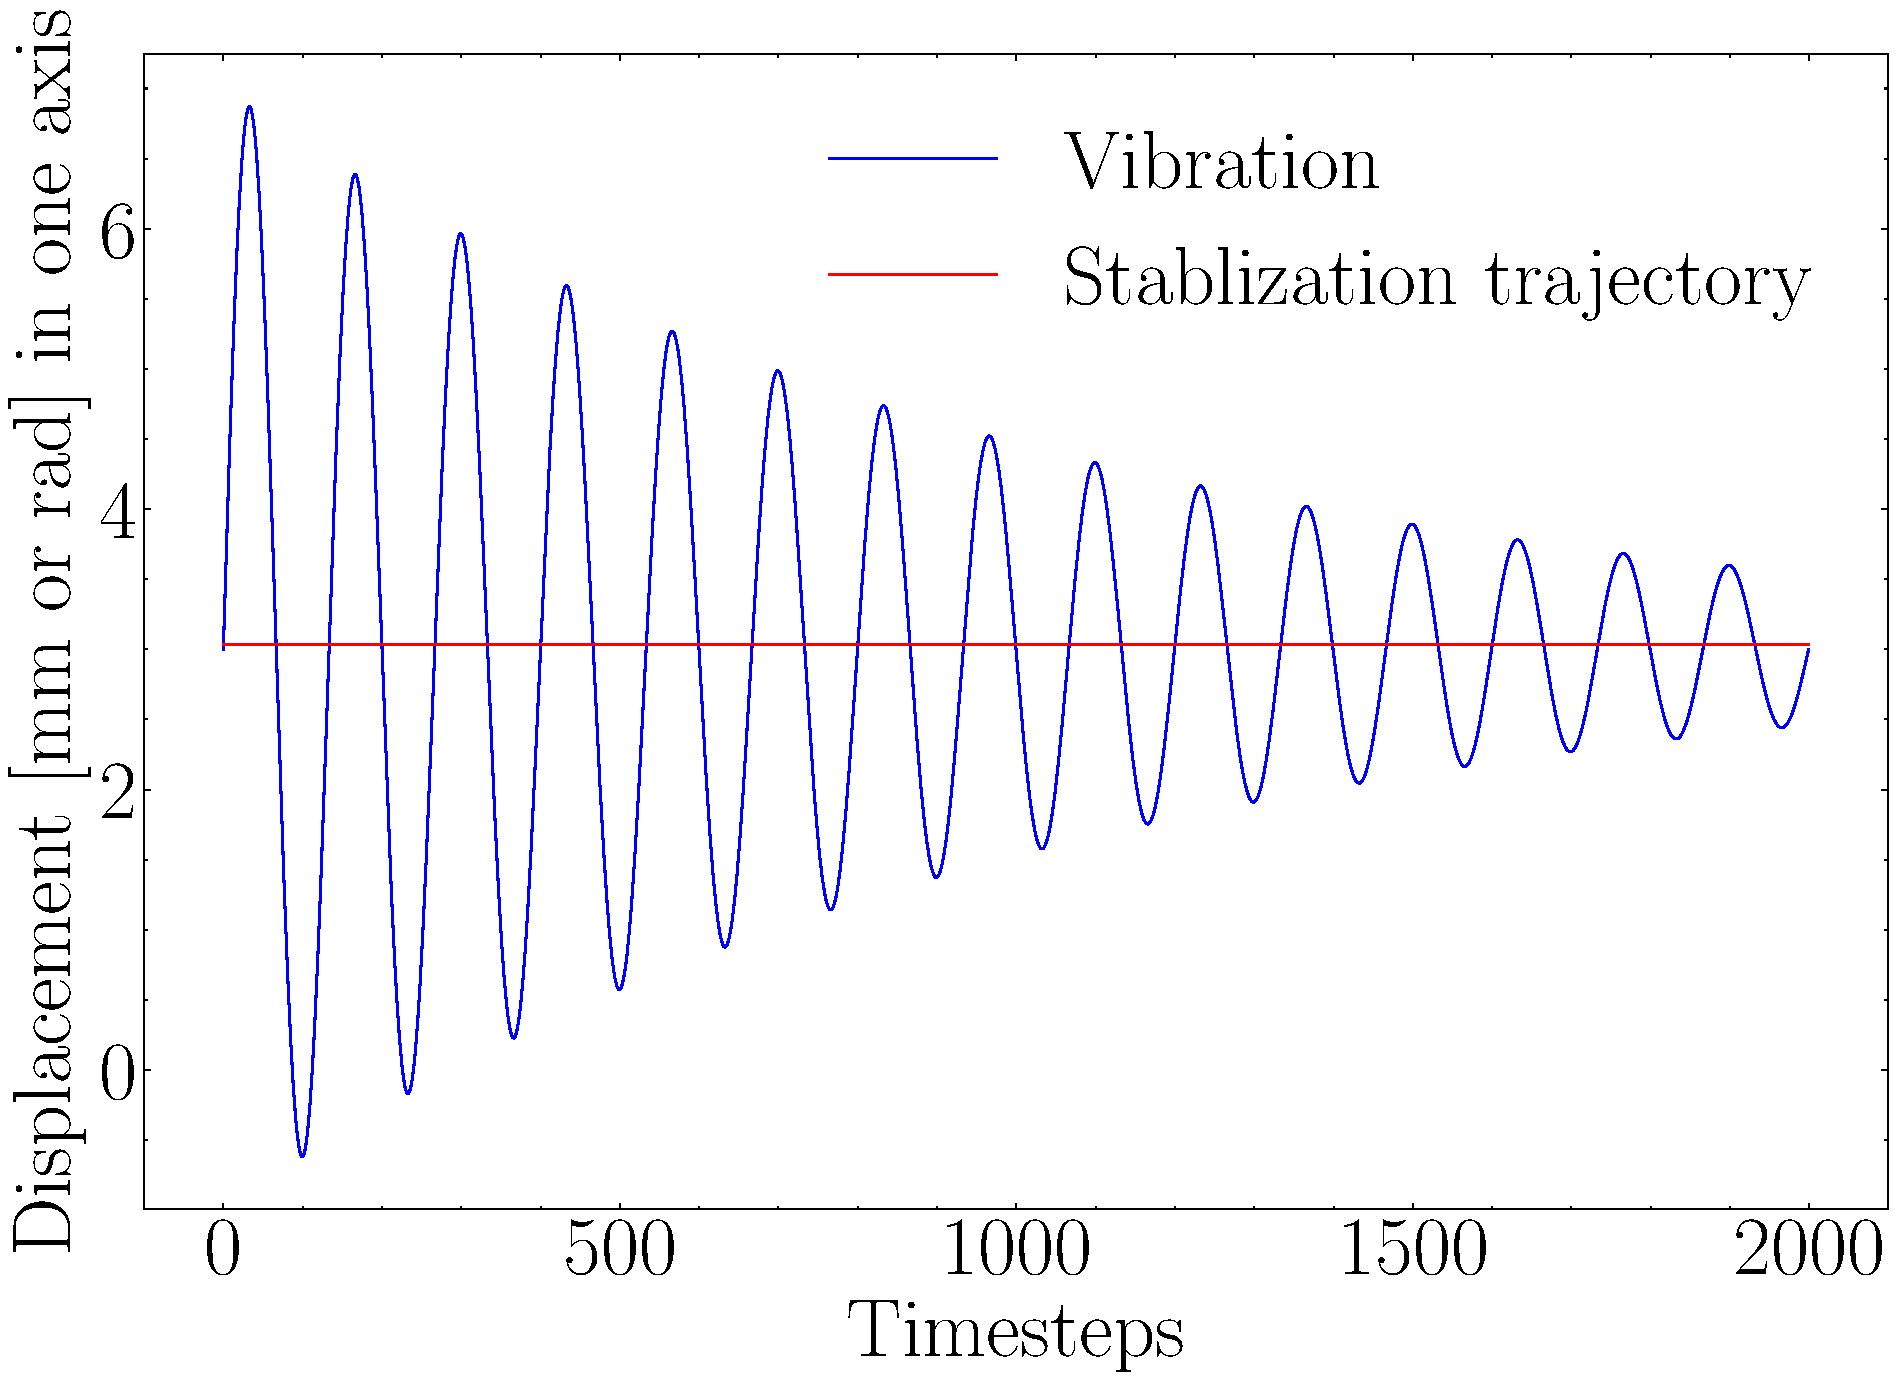
\includegraphics[scale=0.25]{images/fig_chapter2/stab_traj_ideal.pdf}
    \caption{Stabilization Trajectory (Ideal)}
    \label{fig:stab_traj_ideal}
\end{figure}

The size of input to the network is variable based on which if we want to only use Accelerometer readings (3, window-size) or both Accelerometer and Gyroscope sensor readings (6, window-size). The use of accelerometer readings is must because destabilization caused in our use case is mostly due to linear displacements as discussed in chapter section \ref{sec:imu} of this report. 

Various neural network architectures like CNN, MLP, LSTM, ResNet, Transformers and their variations were trained and tested for stabilization trajectory regression. Out of these CNN, ResNet and Transformer architectures had acceptable performance. 

\textbf{Note}: In the next sections I will be only showing neural network outputs plots for translation as the rotation is very small and all the networks correctly predict it with average error in micro-radians range.


%% CNN
\subsection{Convolutional Neural Network}
Convolution neural network with six \textbf{1D-Convolutional} Layers in sequence with \textbf{Batch Normalisation} and  \textbf{ReLU} activation is used to extract features from the input data. Then the output of these convolution layers is regularized using \textbf{dropout} and down-sampled using \textbf{Max-pooling}. Finally, pose is regressed using a series of two fully connected \textbf{Linear} layers.

\begin{figure}
    \centering
    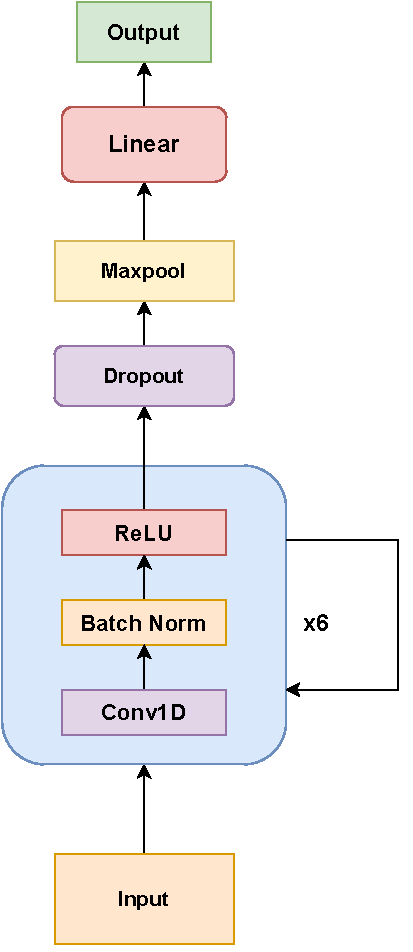
\includegraphics[scale=1]{images/fig_chapter2/nns/cnn_mt.pdf}
    \caption{Convolutional Neural Network Used}
    \label{fig:cnn_used}
\end{figure}

\subsubsection{Model Output Analysis}
Figure \ref{fig:cnn_op_vs_gt} shows the model output vs ground truth plot for a 27 seconds video three linear DoF (x, y, z). The model can regress stabilization trajectory based on input IMU readings with good precision but there are zones where the prediction is off and thus causes jitter in stabilization. The error in all DoF can be seen in figure \ref{fig:cnn_error}.

\begin{figure}[H]
    \centering
    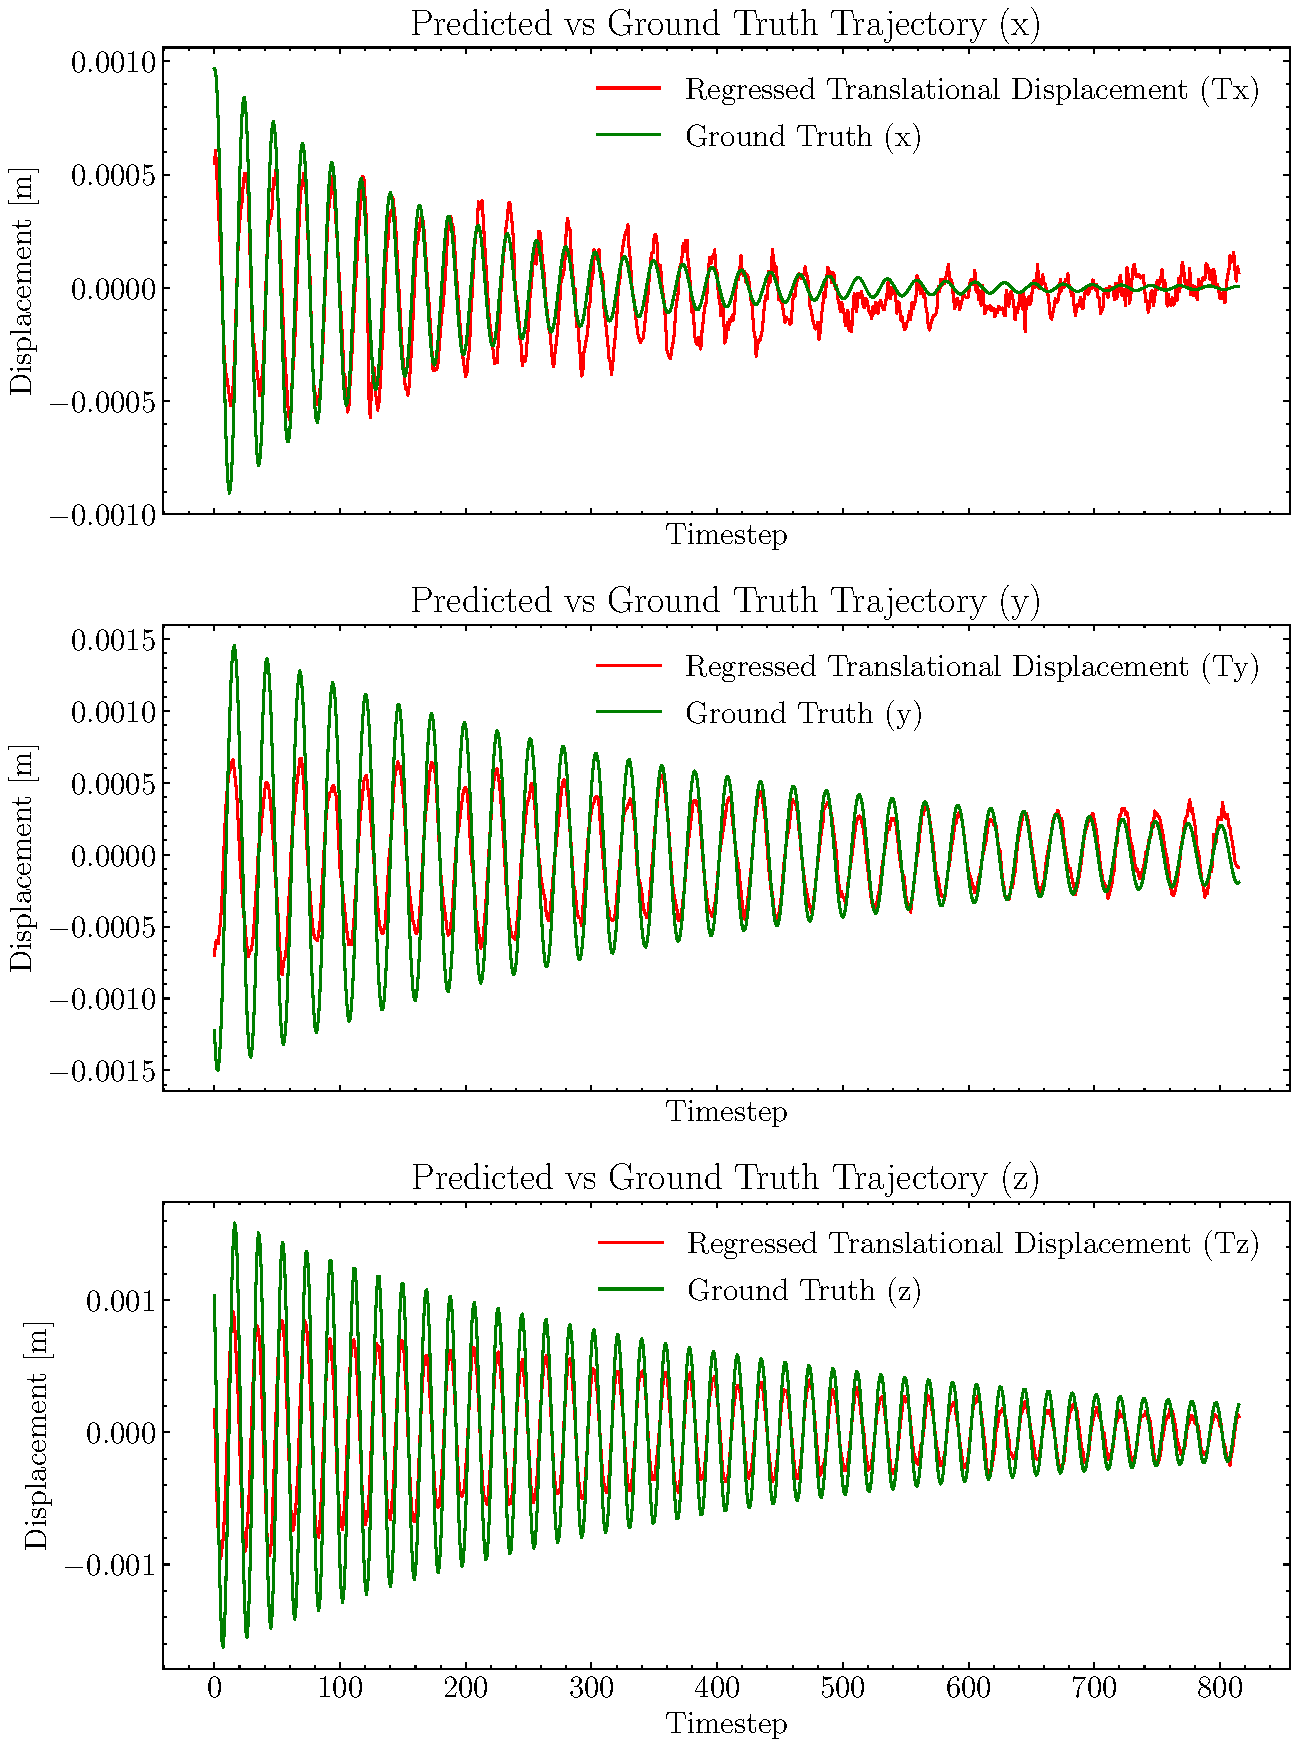
\includegraphics[scale=0.6]{images/fig_chapter4/nn_related/predicted_vs_ground_truth_cnn.pdf}
    \caption{Model Prediction vs Ground Truth for CNN}
    \label{fig:cnn_op_vs_gt}
\end{figure}

\begin{figure}[H]
    \centering
    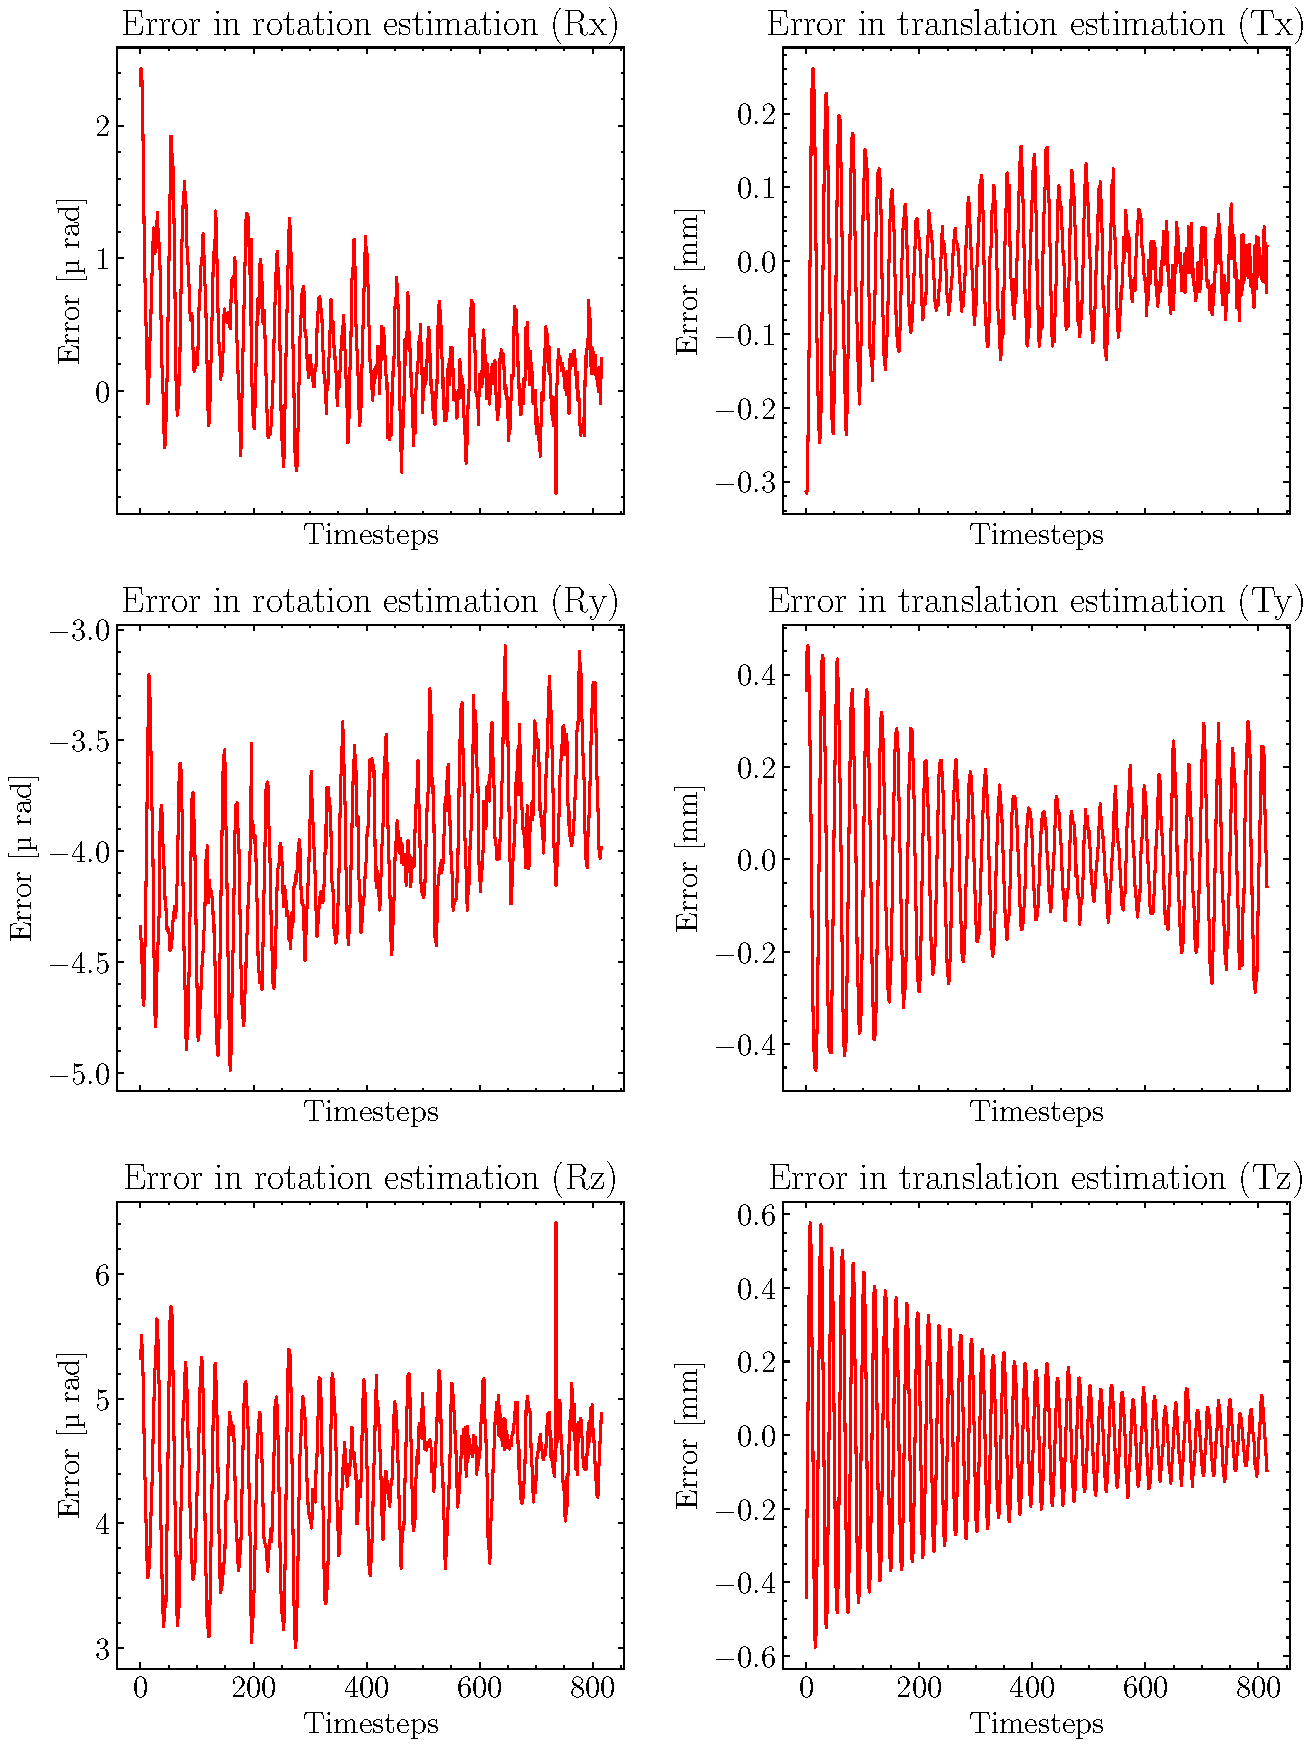
\includegraphics[scale=0.6]{images/fig_chapter4/nn_related/error_in_predicted_vs_ground_truth_cnn.pdf}
    \caption{Error in each DoF for CNN}
    \label{fig:cnn_error}
\end{figure}

%% ResNet
\subsection{ResNet}
Convolution neural network having \textbf{Residual Skip Connections} with six \textbf{1D-Convolutional} Layers in sequence with \textbf{Batch Normalisation} and  \textbf{ReLU} activation is used to extract features from the input data. Then the output of these convolution layers is regularized using \textbf{dropout} and down-sampled using \textbf{Max-pooling}. Finally, pose is regressed using a series of two fully connected \textbf{Linear} layers. 

\begin{figure}[H]
    \centering
    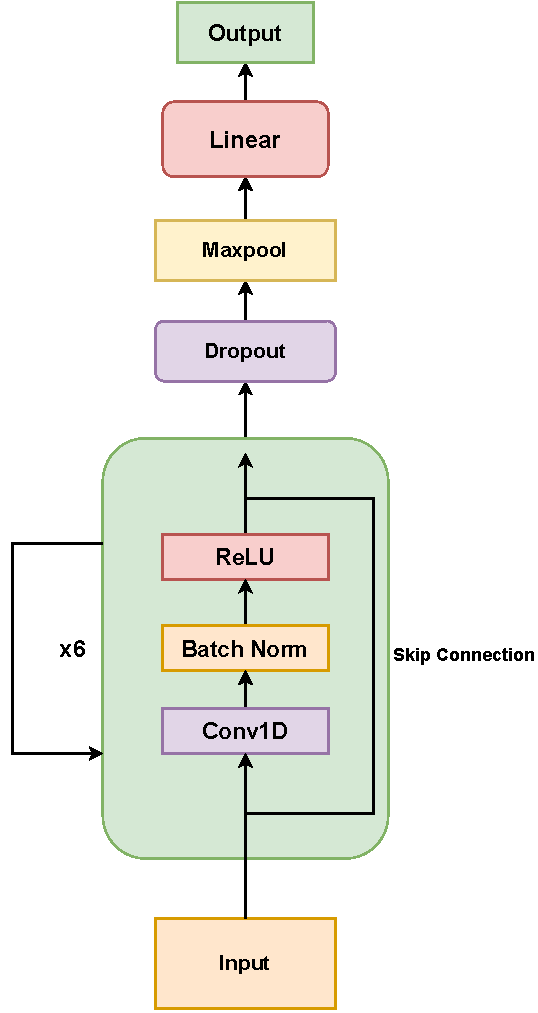
\includegraphics[scale=0.85]{images/fig_chapter2/nns/resnet_mt.pdf}
    \caption{CNN with Residual Skip Connections}
    \label{fig:resnet_used}
\end{figure}

\subsubsection{Model Output Analysis}
Figure \ref{fig:resnet_op_vs_gt} shows the model output vs ground truth plot for a 27 seconds video three linear DoF (x, y, z). The model can regress stabilization trajectory based on input IMU readings with good precision but there are zones where the prediction is off and thus causes jitter in stabilization. The error in all DoF can be seen in figure \ref{fig:resnet_error}.

NOTE: Still under development (Current ResNet model too bulky).

\begin{figure}[H]
    \centering
    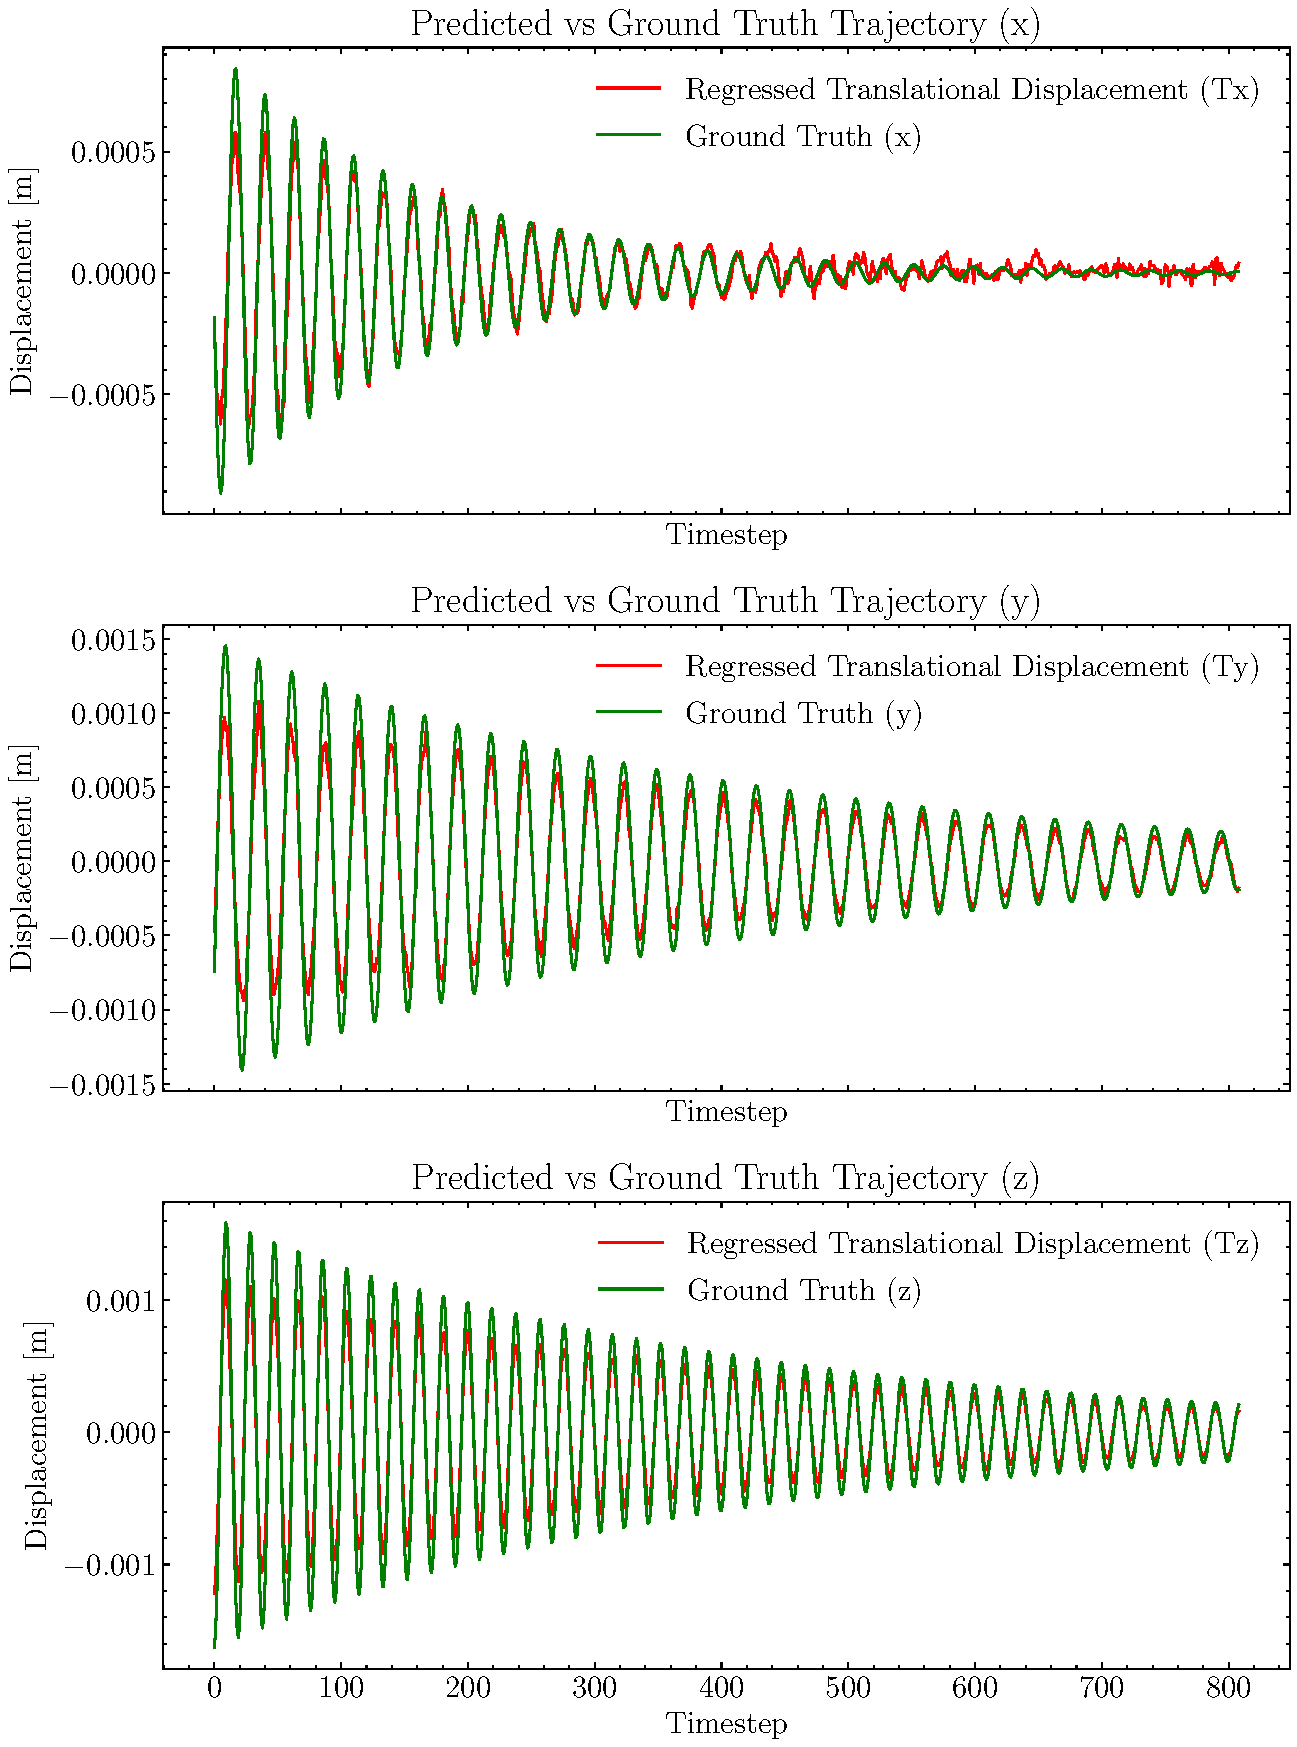
\includegraphics[scale=0.6]{images/fig_chapter4/nn_related/predicted_vs_ground_truth_resnet.pdf}
    \caption{Model Prediction vs Ground Truth for ResNet}
    \label{fig:resnet_op_vs_gt}
\end{figure}

\begin{figure}[H]
    \centering
    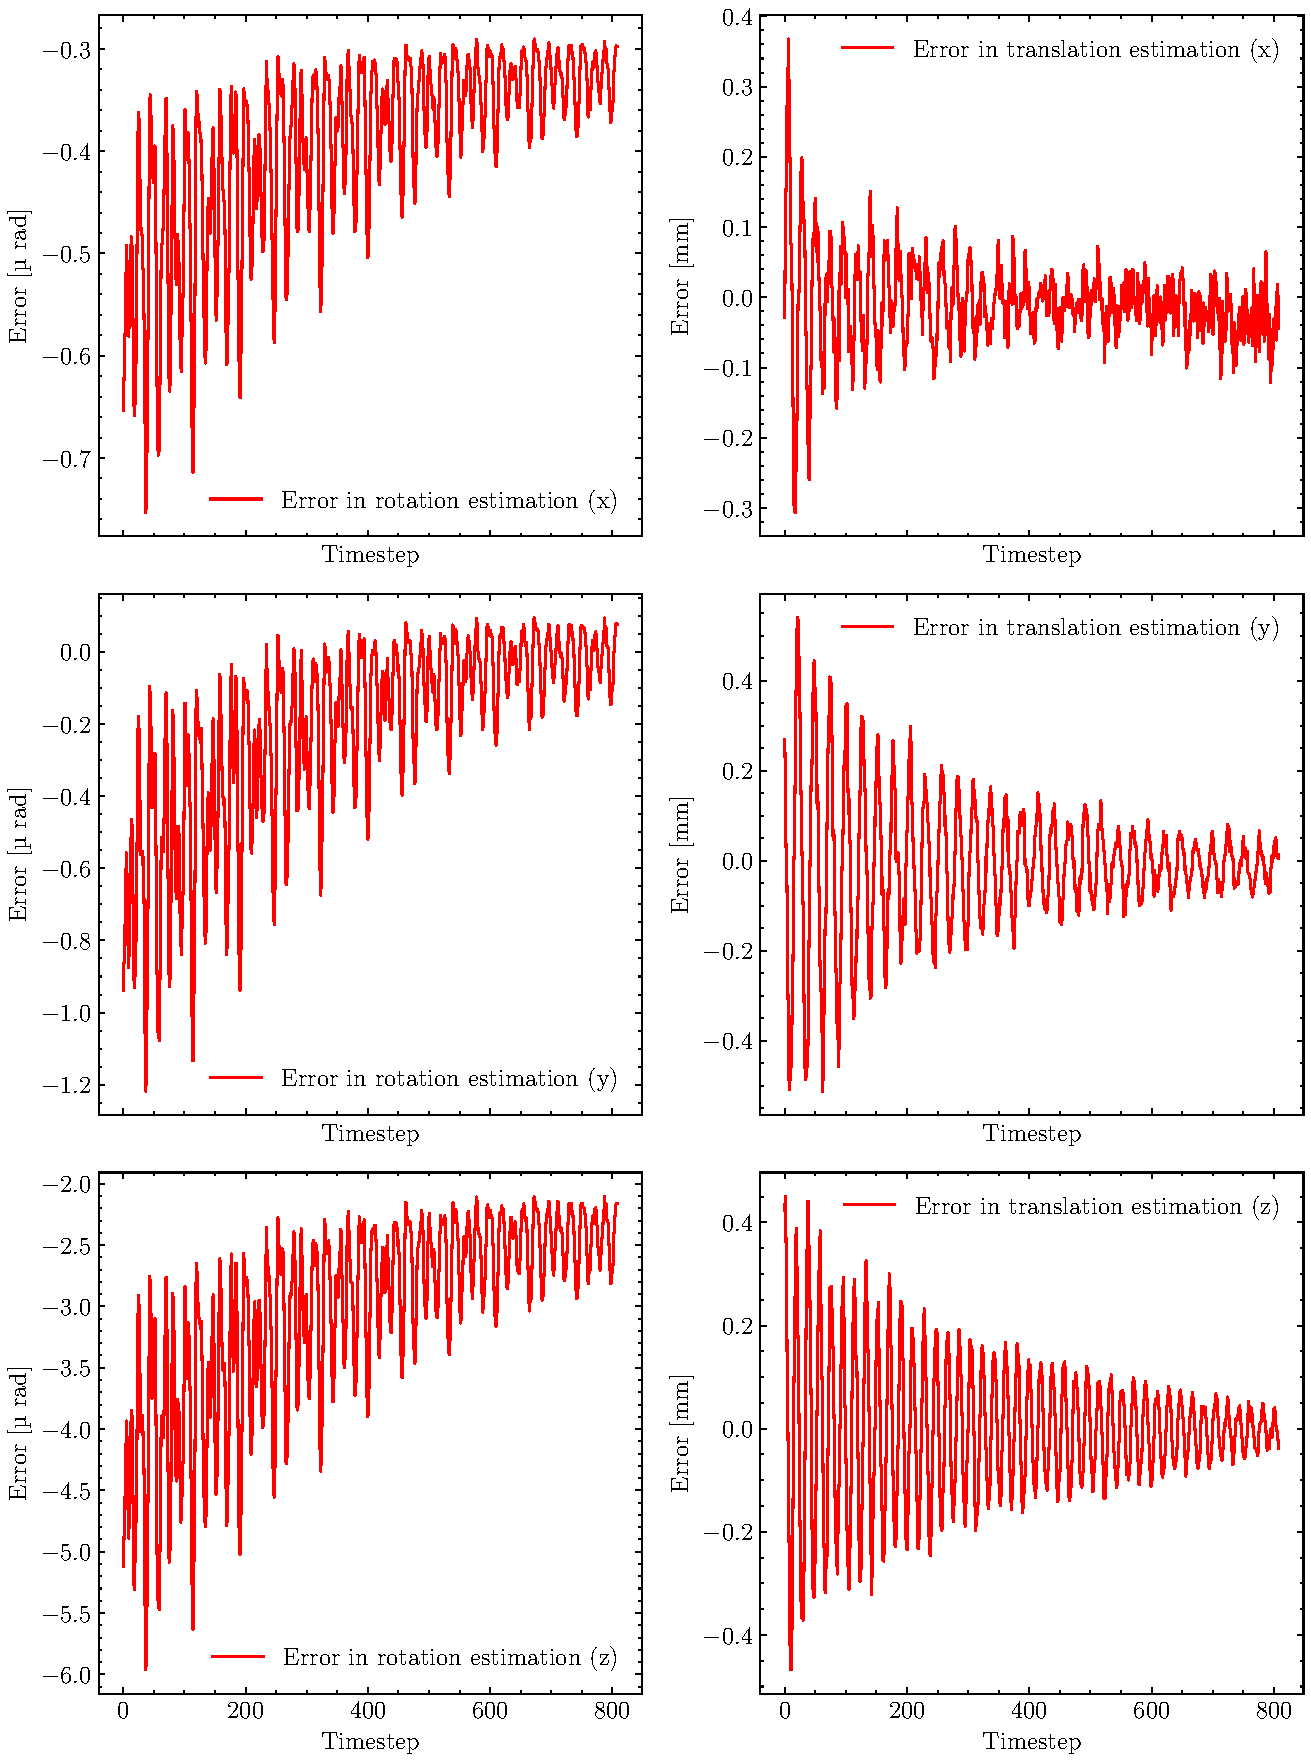
\includegraphics[scale=0.6]{images/fig_chapter4/nn_related/error_in_predicted_vs_ground_truth_resnet.pdf}
    \caption{Error in each DoF for ResNet}
    \label{fig:resnet_error}
\end{figure}


%% CNN-Transformer
\subsection{CNN-Transformer}
The network is structured in a way that the input goes through four \textbf{1D-Convolutional Layers} in sequence with \textbf{GELU} activation (non-linear). The output from these convolutional layers is fed to the \textit{Transformer Encoder}. Transformer Encoder has six layers with each layer having \textbf{Multi Headed Attention}, \textbf{Dropout}, \textbf{GELU} and \textbf{Layer Norm}. The output from the encoder layer goes into the output layers consisting of \textbf{Layer Normalization}, \textbf{Linear} layer, \textbf{GELU} non-linearity, \textbf{Dropout} and finally a \textbf{Fully Connected} layer to regress the output pose.

\begin{figure}[H]
    \centering
    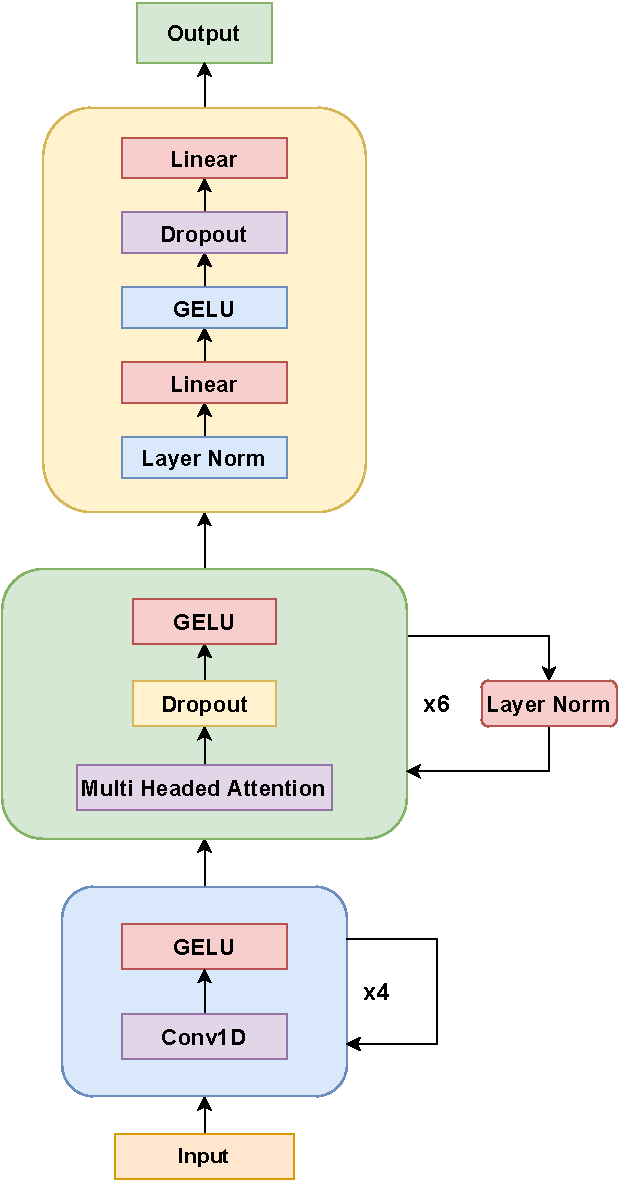
\includegraphics[scale=0.8]{images/fig_chapter2/nns/transformer_mt.pdf}
    \caption{CNN-Transformer Network Used}
    \label{fig:cnn_transformer_used}
\end{figure}

\subsubsection{Model Output Analysis}
Figure \ref{fig:cnn_trans_op_vs_gt} shows the model output vs ground truth plot for a 27 seconds video three linear DoF (x, y, z). The model can regress stabilization trajectory based on input IMU readings with very precision and the error is in a very low range of the order of micrometers ($ \mu m $) and micro radians ($ \mu \theta $).

\begin{figure}[H]
    \centering
    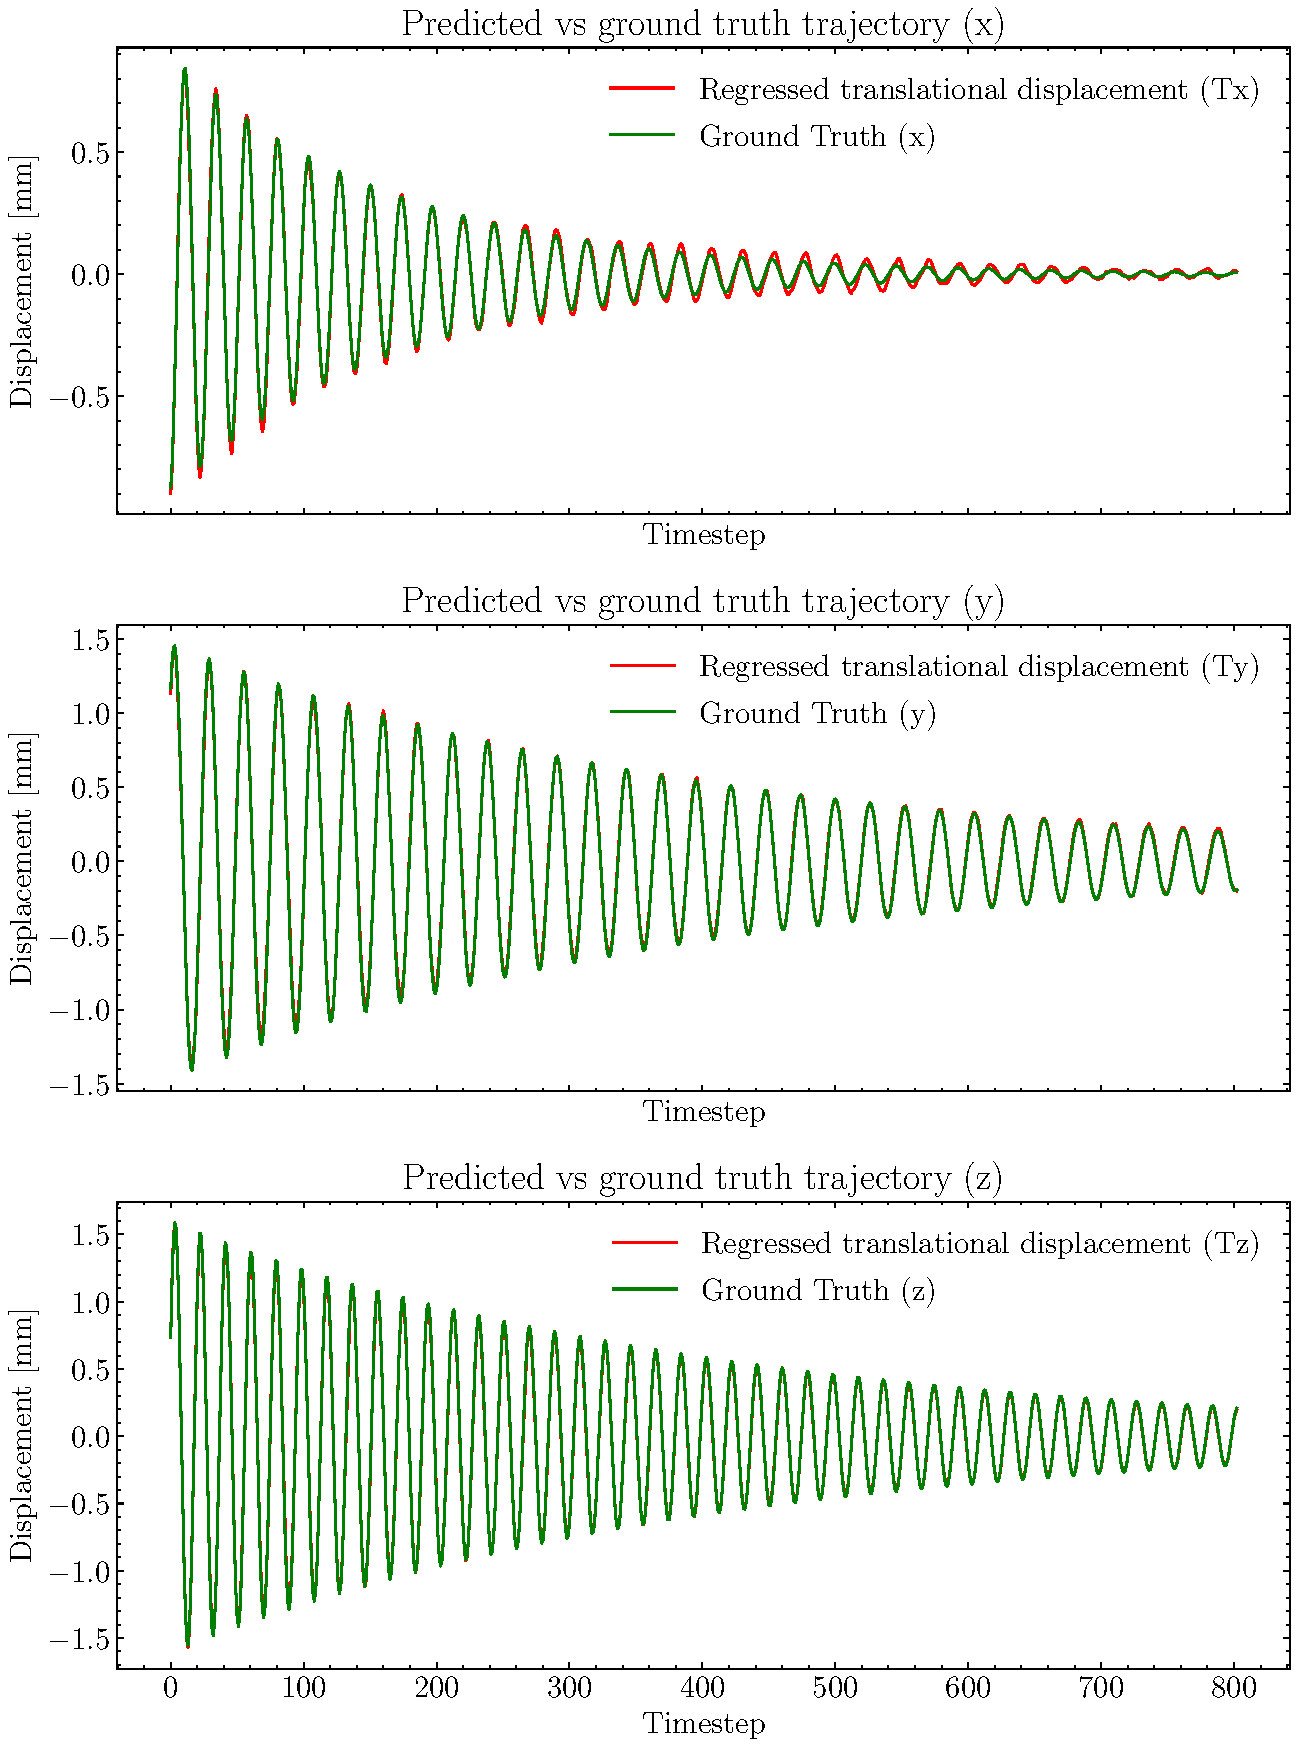
\includegraphics[scale=0.55]{images/fig_chapter4/nn_related/predicted_vs_ground_truth_transformer.pdf}
    \caption{Model Prediction vs Ground Truth for CNN-Transformer}
    \label{fig:cnn_trans_op_vs_gt}
\end{figure}

\begin{figure}[H]
    \centering
    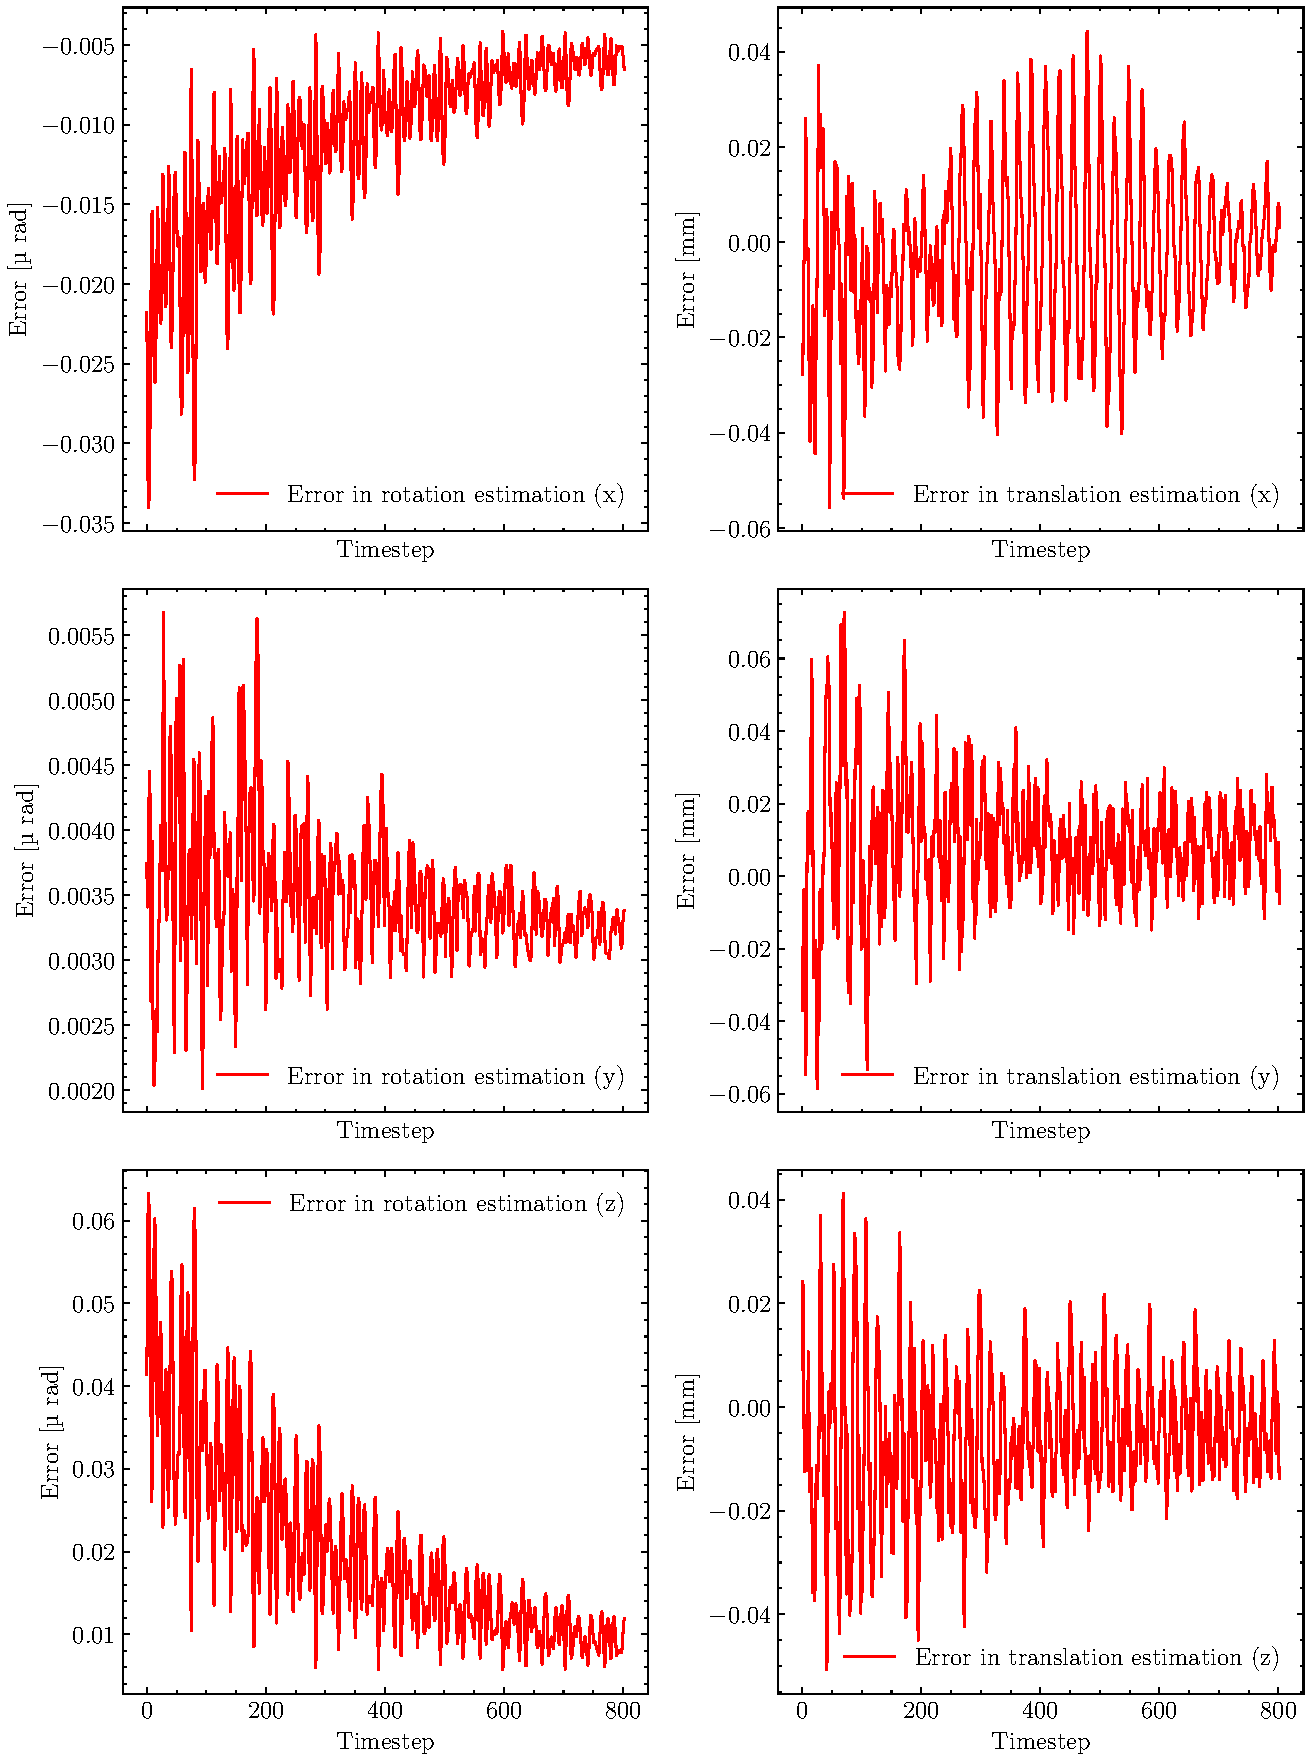
\includegraphics[scale=0.55]{images/fig_chapter4/nn_related/error_in_predicted_vs_ground_truth_transformer.pdf}
    \caption{Error in each DoF for CNN-Transformer Predictions}
    \label{fig:cnn_trans_error}
\end{figure}

\subsection{Smoothening of Stabilization Trajectory}
The neural network is able to regress the stabilization trajectory accurately with the required precision. But the regressed trajectory is not smooth as show in figure \ref{fig:rough_mo_smooth_gt} and has sharp peaks and sudden changes. This is not acceptable as these rough peaks cause jitter in the stabilized video. To account for this, we implemented \textit{Trajectory-Smoothening} in our digital image stabilization pipeline as shown in figure \ref{fig:dis_smooth_pipeline}. An \textbf{Exponential Moving Average Filter} (Equation \ref{eqn:emaf}) is implemented to smoothen the trajectory and minimise jitter. Figure \ref{fig:rough_mo_smooth_mo} shows the effect of this filter on the model output.

\begin{figure}[H]
    \centering
    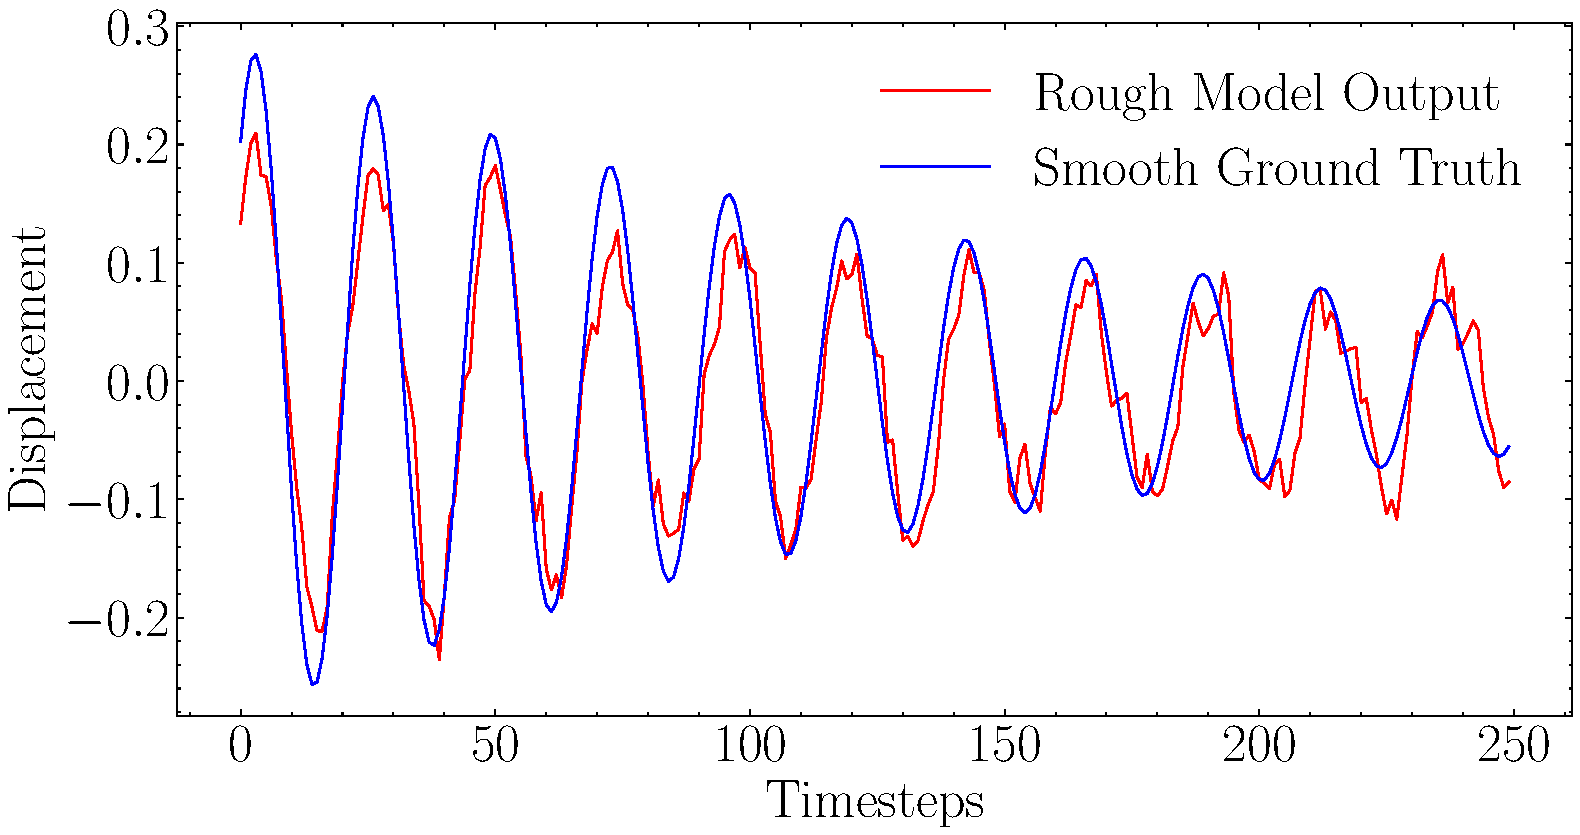
\includegraphics[scale=0.41]{images/fig_chapter4/nn_related/rough_mo_smooth_gt.pdf}
    \caption{Rough regressed vs smooth ground-truth trajectory}
    \label{fig:rough_mo_smooth_gt}
\end{figure}

\begin{equation}[H]
    y_t = x_t  \frac{S}{1+H_l} + y_{t-1}(1 - \frac{S}{1+H_l})
    \label{eqn:emaf}
\end{equation}

Where $ y_t $ is the smoothened signal and $ y_{t-1} $ is the smoothened signal at previous time-step. $ x_t $ is the signal value at current time-step. $ S $ is the smoothening factor and $ H $ is the horizon length. We need to be careful with smoothening the stabilization trajectory because the more we smoothen the higher will be the error introduced in the stabilization trajectory.


\begin{figure}[H]
    \centering
    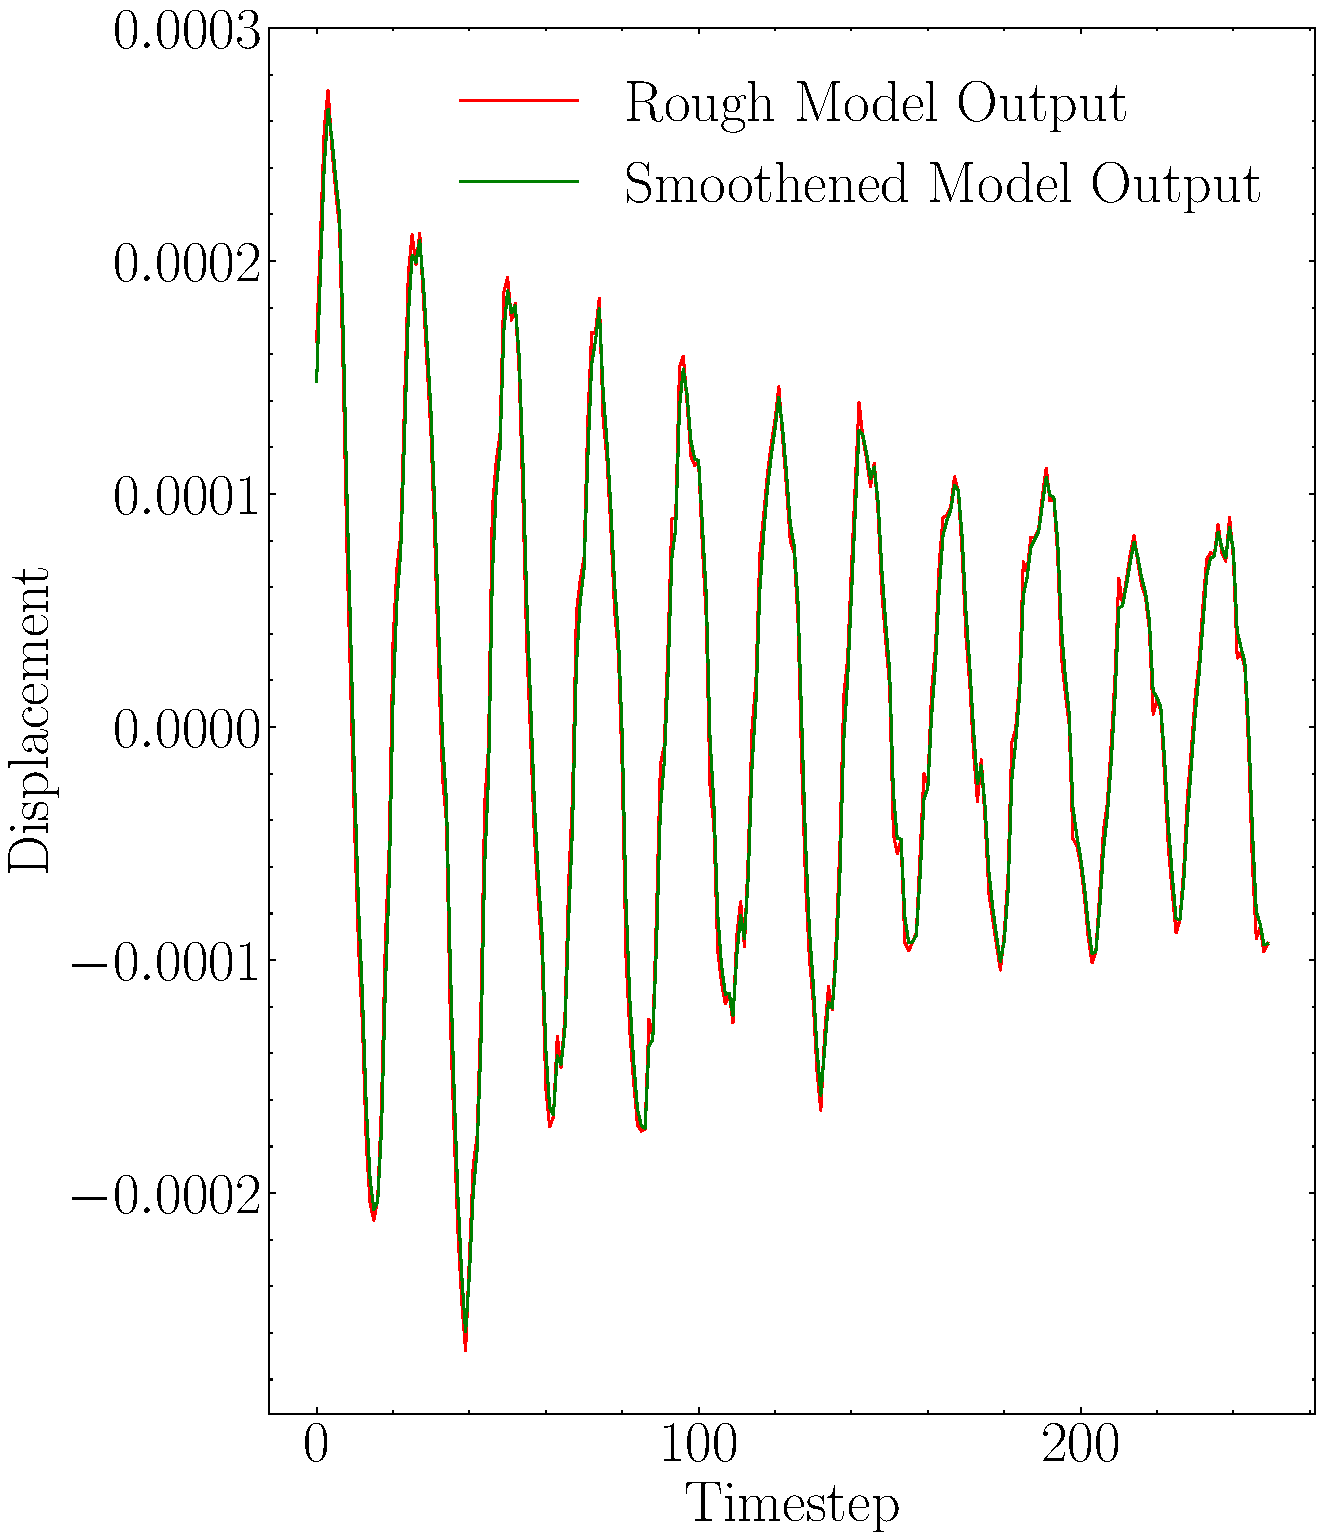
\includegraphics[scale=0.41]{images/fig_chapter4/nn_related/rough_mo_smooth_mo.pdf}
    \caption{Smoothened model output vs raw model output}
    \label{fig:rough_mo_smooth_mo}
\end{figure}

\begin{figure}[H]
    \centering
    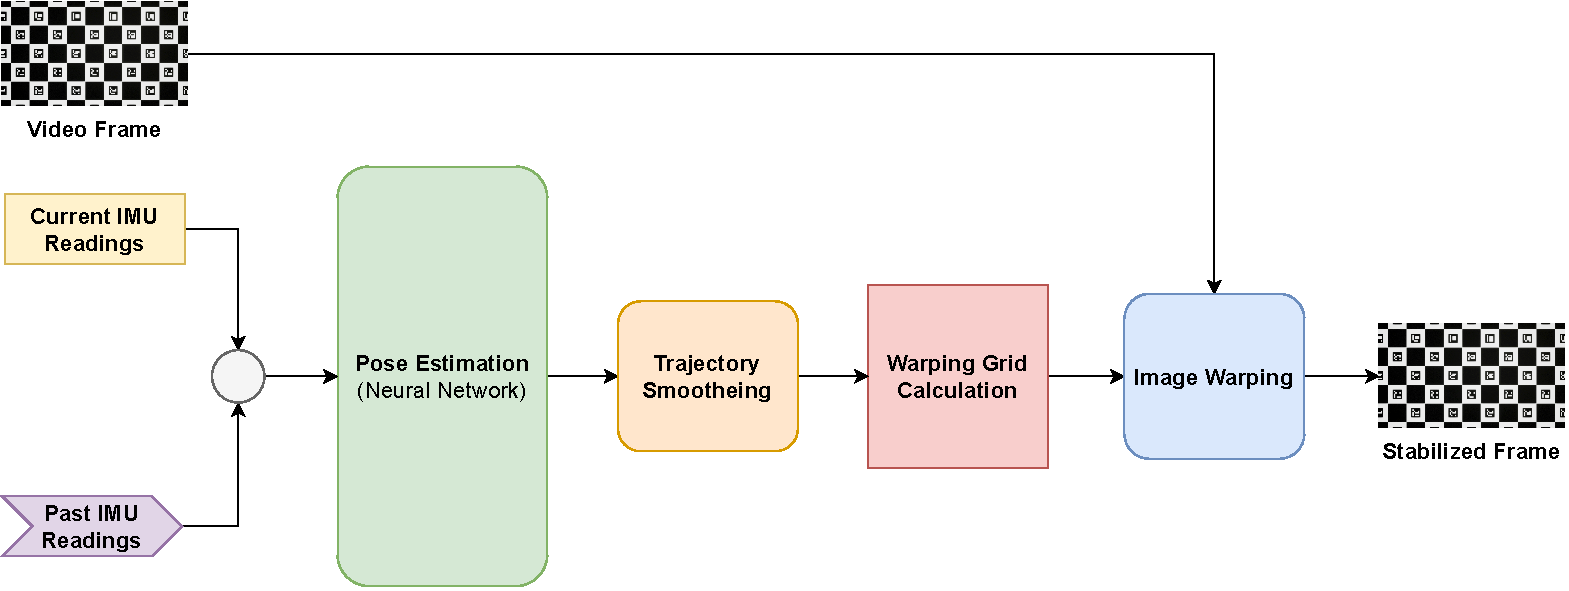
\includegraphics[scale=0.78]{images/fig_chapter4/dis_smooth_pipeline.pdf}
    \caption{DIS Pipeline with Trajectory Smoothening}
    \label{fig:dis_smooth_pipeline}
\end{figure}

\section{Warping Grid Estimation}
In our \textit{Digital Image Stabilization Pipeline} (figure \ref{fig:dis_pipeline}) after getting the relative pose from stabilization trajectory, we need to estimate the warping grid. This warping grid is applied to the image coming from the camera with a crop-ratio of 95 percent (5 percent of the image area will be cropped). These series of warped images based on the pose estimated results into the output stabilized video. 

For warping grid calculation we need to estimate \textit{homography} between stabilized trajectory frame (no actual frame in our case because our prediction is always relative to the stabilized trajectory itself) and the current frame. We assume two image points \textbf{\textit{x}} at times $ t_{i} $ (equation \ref{eqn:x_ti}) and $ t_{j} $ (equation \ref{eqn:x_tj}) from scene points \textbf{X} as shown in figure \ref{fig:dis_point_scene}.

\begin{figure}[H]
    \centering
    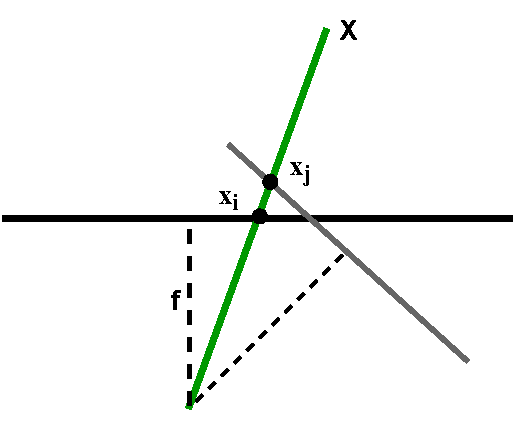
\includegraphics[scale=0.8]{images/fig_chapter4/dis_point_scene.pdf}
    \caption{Scene points at different time-steps}
    \label{fig:dis_point_scene}
\end{figure}

\begin{equation}
    \lambda_{i} x_{i} = K(R(t_i)X + p(t_i))
\label{eqn:x_ti}
\end{equation}

\begin{equation}
    \lambda_{i} x_{j} = K(R(t_j)X + p(t_j))
\label{eqn:x_tj}
\end{equation}

Where, $ R $ is the camera rotation, $ p $ is the camera position and $ K $ is the camera projection matrix (3D to 2D). In our case we have both translation and rotation (although very small). To warp, we need to transform points from camera i to camera j.

\begin{equation}
    \lambda_{i} x_{j} = KR(t_j)R(t_i)^{T} \lambda_{i} K^{-1} x_{i} - K(R(t_j)R(t_i)^{T} p(t_i) + p(t_j))
\label{eqn:homography}
\end{equation}

\begin{equation}
    \lambda_{i} x_{j} = K(R_{rel} \lambda_{i} K^{-1} x_i + p_{rel})
\label{eqn:homography_simplified}
\end{equation}

The relative rotations and translations between two frames (i and j) are estimated using equations \ref{eqn:rel_r} and \ref{eqn:rel_t}. These are the values ($ R_{ij} $ and $ t_{ij} $) neural networks were trained to predict. 

\begin{equation}
R_{ij} = R_i R_i^T
\label{eqn:rel_r}    
\end{equation}

\begin{equation}
t_{ij} = t_i - R_{ij}t_j
\label{eqn:rel_t}
\end{equation}

\section{Model Deployment}
Figure \ref{fig:dis_smooth_pipeline} shows the digital image stabilization pipeline and our goal is to minimise the time taken at each step. The video (images) are coming at 60 FPS from the camera have 4K resolution (3840x2160 pixels). We ideally have 1/60 seconds (16.67 ms) to complete all the steps of the DIS pipeline. In this pipeline, Model Inference and Stabilization grid calculation take most of the given time. Stabilization grid calculation is a series of matrix multiplications and has been already optimized. Thus, low inference latency is highly desirable.

\subsection{Making Models Fast}
There are many techniques to reduce the inference latency of neural network models. Using these methods may reduce the performance of a neural network but are essential for deployment as models in their original form may not be usable at all. Some of the popular methods are discussed below.

\subsubsection{Altering Model Weights}
This is a very common approach used to to tackle high latency of deep learning models especially in case of edge hardware deployment. We can \textbf{quantize} the model by by converting the weights from floating point (32-bits) to integers (8 bits). This decreases the memory requirements significantly while also improving CPU and hardware accelerator latency \citep{FastModels}. 

Another recent approach is to convert the model to \textbf{half-precision} (16-bit floating point). It acts as a middle ground between FP32 and INT8 and the performance trade-off is reduced while decreasing the model size. Another very important thing to note is that not all layers have high latency and thus selective weight altering for layers like convolution layers can also be done making the performance trade-off even smaller.

\subsubsection{Making Models Lean}
The field of deep-learning is growing at a very high rate and we have a large selection of various neural network architectures some even with more than 100 Billion trainable parameters. But while developing deep-learning models, our goal should be to use models with the lowest number of parameters and complex layers while keeping the performance acceptable. The smaller the model is the better its inference latency. 
\subsection{Model Inference Latency on various Hardware}
Various trained models (CNN, ResNet and Transformer) are checked for inference latency and the results are summarised in table \ref{tab:model_inference}. Models were also quantized or converted to ONNX for deployment. The models were inferred 1000 times and the result in the table is an average.

% Sim Vibration characteristics
 \begin{table}[H]
\centering
\begin{tabular}{ l | L | L | L }
    
    Architecture  & 
    Format & 
    No. of Parameters &
    Inference Latency (ms) \\
    \hline
    
    CNN & 
    PyTorch Checkpoint (.ckpt)  & 
    00  &
    00  \\
    
    
    CNN & 
    ONNX (.onnx)  & 
    00  &
    00  \\
    
    ResNet & 
    PyTorch Checkpoint (.ckpt)  & 
    00  &
    00  \\
    
    
    ResNet & 
    ONNX (.onnx)  & 
    00  &
    00  \\
    
    CNN-Transformer & 
    PyTorch Checkpoint (.ckpt)  & 
    00  &
    00  \\
    
    
    CNN-Transformer & 
    ONNX (.onnx)  & 
    00  &
    00  \\

    \hline
   
\end{tabular}
    \caption{Inference Latency of Models}
    \label{tab:model_inference}
\end{table} %%%%


This chapter contained all the steps we took and the techniques we used to successfully realise image invariant digital image stabilization using IMU sensor. We examined various neural network architectures for pose-estimation and as expected more modern architectures outperformed the older neural network architectures. Importance of processing neural network outputs to further improve stabilization was also discussed. 


\section{Results and Discussion}
This section includes a brief overview of everything we have done and the results we have achieved.

\begin{itemize}
    \item Digital Image stabilization was chosen to stabilize the video for our use case as hardware stabilization is expensive and bulky with a lot of moving parts.

    \item Camera motion estimation was achieved using MEMS IMU sensor due its low price and high reliability.

    \item Use of MEMS IMUs present a huge challenge in accurate pose estimation as the noise characteristics of IMU along with the use of classical inertial navigation algorithm makes it impossible to accurately estimate pose accurately. Even the use of advanced state estimation algorithms is futile.

    \item Both real world and simulated data was collected to train the neural networks and test the image stabilization algorithm.

    \item Data-driven approaches like RoNIN(CNN and ResNet) were tested to estimate camera pose accurately and showed promising results over classical approaches.

    \item More advanced self-attention based neural network architectures were used (CNN-Transformer) which improved the accuracy of stabilization trajectory estimation to a very high level.

    \item This resulted into very good IMU based digital image stabilization.

    \item Outputs from the neural networks were not smooth causing some jitter in the stabilized video.

    \item Exponential moving average filter was used on neural network outputs to smoothen the predicted trajectory and improve the quality of video stabilization even more.

\end{itemize}


\subsection{Future Work}
\begin{itemize}
    \item Adapt this stabilization technique to high field of view and low focal length camera setups.

    \item Explore lean neural network architectures to obtain similar results with low latency networks that are deploy-able on cheaper hardware.

    \item Figure out way to use semi-supervised or unsupervised learning techniques to eliminate the hassle of ground truth generation.
    
\end{itemize}
